% options:
% thesis=B bachelor's thesis
% thesis=M master's thesis
% czech thesis in Czech language
% english thesis in English language
% hidelinks remove colour boxes around hyperlinks

\documentclass[thesis=M,english,hidelinks]{FITthesis}[2012/10/20]

\usepackage[utf8]{inputenc} % LaTeX source encoded as UTF-8
% \usepackage[latin2]{inputenc} % LaTeX source encoded as ISO-8859-2
% \usepackage[cp1250]{inputenc} % LaTeX source encoded as Windows-1250

\usepackage{graphicx} %graphics files inclusion
\usepackage{csquotes}
% \usepackage{subfig} %subfigures
% \usepackage{amsmath} %advanced maths
% \usepackage{amssymb} %additional math symbols

\usepackage{dirtree} %directory tree visualisation

\usepackage{csvsimple}
\usepackage{longtable}
\usepackage{multicol}
\newsavebox\ltmcbox

\usepackage[table]{xcolor}
\usepackage{placeins}

\usepackage{listings}
\lstdefinestyle{default}{
	basicstyle=\ttfamily,
	breaklines=true,
	breakatwhitespace=true,
	breakindent=0pt
}
\lstdefinestyle{filestyle}{
	basicstyle=\footnotesize,       % the size of the fonts that are used for the code
	%numbers=left,                   % where to put the line-numbers
	%numberstyle=\tiny,              % the style that is used for the line-numbers
	%numbersep=5pt,                  % how far the line-numbers are from the code
	frame=single,                   % adds a frame around the code
	tabsize=4,                      % sets default tabsize to 2 spaces
	captionpos=b,                   % sets the caption-position to bottom
	breaklines=true,                % sets automatic line breaking
	breakatwhitespace=false,        % sets if automatic breaks should only happen at whitespace
	postbreak=\mbox{$\hookrightarrow$\space},
}
\lstset{style=default}

% % list of acronyms
% \usepackage[acronym,nonumberlist,toc,numberedsection=autolabel]{glossaries}
% \iflanguage{czech}{\renewcommand*{\acronymname}{Seznam pou{\v z}it{\' y}ch zkratek}}{}
% \makeglossaries

\newcommand*{\qt}[1]{\enquote{{\itshape#1}}}
\newcommand*{\lstfile}[3]{\lstinputlisting[style=filestyle, firstnumber=#2, firstline=#2, lastline=#3, caption=#1]{listings/#1}}

\makeatletter
\renewcommand\@makefntext[1]{\leftskip=2em\hskip-2em\@makefnmark#1}
\makeatother

\newcolumntype{C}{>{\centering\arraybackslash}X}
\newcolumntype{R}{>{\raggedleft\arraybackslash}X}

% % % % % % % % % % % % % % % % % % % % % % % % % % % % % % 
% EDIT THIS
% % % % % % % % % % % % % % % % % % % % % % % % % % % % % % 

\department{Department of Theoretical Computer Science}
\title{Record and Replay debugging in R}
\authorGN{Kryštof} %author's given name/names
\authorFN{Slavík} %author's surname
\author{Kryštof Slavík} %author's name without academic degrees
\authorWithDegrees{Bc. Kryštof Slavík} %author's name with academic degrees
\supervisor{Ing. Petr Máj}
\acknowledgements{
	I would like to thank my supervisor Ing. Petr Máj for all the help given during the course of writing this thesis.\par
	Thanks to members of PRL-PRG lab for their insight into R given on several occasions.\par
	Special thanks go to Tomáš Nováček for proofreading the text.\par
	And last but not least, I thank my family for being supportive throughout my studies.\par
}
\abstractEN{
	Non-determinism in programs often causes unwanted behaviour to appear and disappear seemingly randomly. Record and Replay debugger is a tool which helps programmers to isolate such behaviour by recording a program's execution once when the bug appears and then replaying it later multiple times in the exact same way with the bug present while providing classic debugging facilities. This thesis focuses on implementation and integration of such tool into R programming language which is commonly used in mathematics, mainly in statistics.
}
\abstractCS{
	Nedeterminismus v programech často způsobuje, že se v nich nežádoucí chování vyskytuje zdánlivě náhodně. Record and Replay debugger je nástroj, který umožňuje programátorům izolovat takové chování tím, že se běh programu nahraje jednou ve chvíli, kdy k výskytu bugu dojde, a následně se vícekrát naprosto stejným způsobem přehraje za neustálé přítomnosti tohoto bugu včetně možnosti použití klasických debuggovacích nástrojů. Tato práce se zaměřuje na implementaci a integraci takového nástoje do programovacího jazyka R, který se běžně používá v matematice, zejména ve statistice.
}
\placeForDeclarationOfAuthenticity{Prague}
\keywordsCS{Record and Replay debuggování, deterministické debuggování, tracing, programovací jazyk R}
\keywordsEN{Record and Replay debugging, deterministic debugging, tracing, R language}
\declarationOfAuthenticityOption{1} %select as appropriate, according to the desired license (integer 1-6)
\website{https://github.com/krystofslavik/RRnR} %optional thesis URL


\begin{document}

% \newacronym{CVUT}{{\v C}VUT}{{\v C}esk{\' e} vysok{\' e} u{\v c}en{\' i} technick{\' e} v Praze}
% \newacronym{FIT}{FIT}{Fakulta informa{\v c}n{\' i}ch technologi{\' i}}

\setsecnumdepth{part}
\chapter{Introduction}\label{introduction}
\vspace{-10pt}
A non-deterministic bug in software is an unwanted behaviour which happens with a low probability. Such bugs are not easily observable and thus are very hard to fix. Usually the program works flawlessly and is seemingly perfect until an error occurs under a certain set of conditions. This most likely happens during normal usage and it is witnessed by a common user, not a developer. It is practically impossible for the developers to find the bug with the basic information provided by the user so the only viable option is to try to reproduce the problem. This might take a lot of time depending on the probability of the bug's occurrence.\par

Usually a bug can be detected by its symptoms but that is not enough to find its origin. Developers need a way to reproduce it many times in order to understand it properly. During normal debugging session the main symptom and its direct cause are found first. In the second run a cause of the cause is revealed and so on until the real source of the problem is discovered. In each run it is possible to trace the chain of symptoms only a few steps back because the program cannot be run backwards. This approach is tedious but it provides the result eventually.\par

However, finding non-deterministic bugs this way is even more tedious and therefore much harder. As the bug appears only with a certain probability it is necessary to run the program $n$ times in order to trigger it and this process must be repeated for each of the $m$ steps needed to get from the final symptom to the root cause which brings the total number of runs necessary from $m$ to $n*m$~\cite{fitzgerald}.\par

The discovery of non-deterministic bugs may be improved if they could be reliably reproduced. Doing so effectively transforms them into deterministic bugs and the standard approach may be used. This can be achieved by recording all the varying information contained in the program which causes the bug to appear. Typically this might be user input, network packets, filesystem contents but also the state of a random number generator, etc. With this information it is theoretically possible to re-run the program in the exact same way every time.\par

The problem is illustrated by the following example program which calculates an average tangent value of a set of angles. Built-in \lstinline|tan()| function in R only works with radians so there are three helper functions implemented which calculate the tangent manually from degrees. The input angles are generated randomly in the range from 0 to 180 degrees but in reality they might be read from a user input or another non-deterministic source as well, the point is that they are different in each run.\par

\begin{lstlisting}[style=filestyle, caption={The program containing a non-deterministic bug}, label=example_program]
tangent <- function(y, x) y/x
adjacent <- function(a, c) cospi(a / 180.0)*c
opposite <- function(a, c) sinpi(a / 180.0)*c

scale <- 100
angles <- floor(runif(100, min=0, max=180*scale))/scale

tangents <- c()
for(i in 1:length(angles)) {
  adj <- adjacent(angles[i], 1)
  opp <- opposite(angles[i], 1)
  tan <- tangent(opp, adj)
  tangents[i] <- tan
}

return(mean(tangents))
\end{lstlisting}

The program contains a non-deterministic bug -- in rare occasions it outputs \lstinline|Inf| (which stands for infinity) instead of a real number. By conventional means it is hard to find the bug in this simple example and it is even harder to do so in a large real-world program. This thesis presents a tool called \emph{RRnR} which allows for easier debugging of such programs and the results of debugging this program with RRnR are shown in the last chapter.\par

RRnR records an execution of a program written in R and then allows the user to replay the execution many times in the exact same way. Furthermore it allows standard debugging tools to be used during the replaying and it provides functions which make it more easy to detect the bug for the first time. The R programming language is commonly used in mathematics, mainly in statistics, and therefore the tool has a large number of potential users who might benefit from it.\par

The \emph{first chapter} of this thesis describes the record and replay debugging in more depth and presents its existing implementations. In the \emph{second chapter} the R programming language is introduced and its main functionality is presented along with important details of its implementation. The implementation details of RRnR are written in the \emph{third chapter}. Also the entire functionality of the tool is described there. In the \emph{final chapter} the functionality of the tool is evaluated in a series of benchmarks and real-world tests.\par

\setsecnumdepth{all}
\chapter{Record and Replay debugging}
Record and Replay debugging (RR) is a solution for making debugging of non-deterministic bugs simpler. RR extends classic program debugging tools like GDB\footnote{GDB -- GNU Debugger, \url{https://www.gnu.org/software/gdb/}} by \qt{recording the non-deterministic events of a program’s execution in a log, and later using the log to replay the program deterministically. The typical non-deterministic events that are logged are the inputs to the program (such as system call return values and side effects, and signals) and the memory access interleavings of the threads.}~\cite{RnR}\par

With RR it is possible to record the program execution once and then replay the recorded program over and over in the exact same way while using standard debugging tools for inspecting the code and memory. This feature alone speeds up the debugging process significantly depending on how often would the bug appear in a normal debugger.\par

Some of the RR debuggers also have the ability to reverse execute the program which means that it is not only possible to step through the program forwards but also a step back can be made. The reverse execution may speed up the debugging process even more and it may also be useful for debugging deterministic bugs as well.\par

There have been several implementations of RR, many of them based on running a whole operating system inside a virtual machine (VM). Besides QIRA~\cite{qira} which uses an opensource computer emulator QEMU\footnote{QEMU -- Quick EMUlator, \url{https://www.qemu.org/}}, the most notable is RR implementation in VMware Workstation\footnote{VMware Workstation -- virtualization software,\par\url{https://www.vmware.com/products/workstation-pro.html}} which in combination with Visual Studio\footnote{Visual Studio -- programming IDE, \url{https://www.visualstudio.com/}} allowed to run RR debugging~\cite{vmware}.\par

Using virtualization in the context of RR has many advantages. In order for the RR to work it is necessary to create a barrier between deterministic code execution and non-deterministic outside influence. The virtual machines are already doing that as they are themselves completely deterministic and all the non-determinism which comes from I/O communication is separated by the virtualization interface. This means that when a copy of the machine's inner state is made and then used later the behaviour of the machine will be exactly the same with the exception of the I/O communication which can be relatively easily recorded as well.\par

However, the biggest disadvantage of such approach lies in the large runtime overhead caused by virtualization of the entire machine. VMs are also extremely complex and adding even more complexity in form of the RR implementation is very difficult. Mainly because of the complexity reasons VMware decided to discontinue development of their RR~\cite{vmware_end}.\par

There is also another approach. Mozilla developed their easy-to-use low-overhead RR debugger which does not need to virtualize the whole OS and is built on top of a well known debugger GDB~\cite{rr}. Not using a virtualization software is clearly an advantage, mainly because of the performance benefits. On the other hand all the features that are recorded and replayed in the VMs easily, like thread synchronization, OS event timing, process interaction, etc., have to be controlled explicitly or are even impossible to control in this method.\par
		
	\section{Mozilla rr}
	% http://jakob.engbloms.se/archives/2306
	% http://fitzgeraldnick.com/2015/11/02/back-to-the-futurre.html
	% https://www.youtube.com/watch?v=ytNlefY8PIE
	Developers at Mozilla were facing some difficulties with bugs appearing only in certain situations which made them difficult to debug using standard debuggers~\cite{rr_vid}. They realized that they could use some form of RR debugging, however none of the existing tools were sufficient because of their complexity and poor performance. Finally they decided to create their own tool with a few simple (but nontrivial) goals in mind~\cite{rr}:
	\begin{itemize}
		\item \emph{Easy to deploy}\par
			It should run directly on the user's OS and hardware. No need to change system configuration.
		\item \emph{Low run-time overhead}\par
			Slowdown caused by the debugger should be as low as possible.
		\item \emph{Simple}\par
			Mozilla had very limited resources so they avoided building complex solutions.
		\item \emph{Compatible with Firefox}\par
			The primary goal was to debug Firefox, however rr works with other applications too.
	\end{itemize}
	
	All of the goals were met and especially the simplicity of use and very low overhead puts Mozilla rr ahead of any other RR solution. Depending on workload rr can achieve slowdown of as low as 20\% and in most cases it is much faster than any other competing technology~\cite{rr}.\par
	
	The actual performance degradation depends mainly on the number of system calls that the recorded application makes. More syscalls usually mean slower recording but on the other hand the more calls are recorded the less is left to actually execute in the replay phase. If, for instance, the application downloads a big file from the Internet then the replay phase is much faster as the file is not being downloaded at all.\par
	
	There are naturally some limitations to the rr as well. It emulates a single-core machine which significantly reduces performance of multithreaded applications. It cannot record processes which share memory with other non-recorded processes. And finally it heavily depends on features in Linux kernel and Intel CPUs and therefore it cannot be used on other platforms.\par
		
		\subsection{Internals of Mozilla rr}
		This is a quick overview of how the most important parts of rr work based on Robert O'Callahan's talk at Linux.conf.au 2016~\cite{rr_vid} and slides at rr's web page~\cite{rr_slides}.
		
		Mozilla rr records non-deterministic events during program's execution which are system call (syscall) results and signals. To achieve this it uses the \emph{ptrace} system call in Linux which allows inspecting child processes. With \emph{ptrace} rr is notified before and after every syscall made by the monitored program. Using \emph{ptrace}, however, causes some slowdown as it introduces several context switches for each syscall. To avoid this unnecessary overhead the most common syscalls are instead wrapped with a code, which performs the recording, injected directly into the monitored program.\par
		
		Multithreaded programs are run only in one thread in order to avoid temporal non-determinism which cannot be properly recorded.\par
		
		A normal program execution is sometimes interrupted by various signals like \emph{SIGALARM}. Source of the signals is considered to be non-deterministic as they are generated by the OS. Therefore they must be recorded and replayed which can be done relatively easily, but the main problem is replaying them at the right time. For this rr uses retired conditional branches counter (where retired basically means executed) which is one of hardware performance event counters (HPCs).\par
		
		HPCs are parts of the CPU which can count executed instructions, branches, etc. and can be programmed to stop the execution after a certain value is reached. When recording, the counters are programmed to stop after every $k$ steps. If during the elapsed time a signal has been received then it is recorded along with the current value of the counter. Finally during replay the counter is programmed to trigger the recorded signals after the recorded number of events which replays them \emph{roughly} at the right time. However, different CPUs have different HPCs and HPCs used by the rr are only present on newer (at least Nehalem architecture) Intel CPUs.\par
		
		Another problem occurs when there is a blocking syscall waiting for another thread. As rr runs only one thread at a time it needs to detect this situation in order to avoid deadlock and switch to the other thread. The problem is that once the blocking syscall is made the control is never returned to rr by default. This can be solved by using \emph{DESCHED} performance event which generates a \emph{SIGSYS} signal every time the OS does a context switch. Receiving the \emph{SIGSYS} signal causes an interrupt and an execution of a handler which is registered by rr. Which means that rr gets the control and can act accordingly. The \emph{DESCHED} event is registered right before a blocking syscall is made and it is unregistered right after the syscall is done so that it does not cause any \qt{false alarms}.\par
		
		To be able to actually debug the program rr uses GDB. All features of GDB are supported including running an arbitrary function in the program being debugged. However, running this function was not part of the recorded run, therefore it cannot be replayed. Because of that rr forks the process, then runs the function, collects the output, terminates the forked process and resumes the original process.\par
		
		Another feature is the ability to reverse-execute. During forward execution the debugger saves checkpoints. Then during backward execution the debugger jumps back to the nearest checkpoint and from there continues forward until it reaches the target place.\par

	\section{QIRA}
	% https://bananaappletw.github.io/2016/03/22/qira-introduction/
	% https://github.com/BinaryAnalysisPlatform/qira
	% http://qira.me/
	% https://www.haikudeck.com/timeless-debugging-education-presentation-0f7bc40fb2#slide1
	% https://www.youtube.com/watch?v=eGl6kpSajag
	As stated above, Mozilla rr is not the only RR solution. There are (or have been) other RR debuggers, mostly based on some kind of virtualization. One of such RR debuggers is QIRA~\cite{qira} (QEMU Interactive Runtime Analyser). This debugger is created in Python\footnote{Python -- interpreted programming language, \url{https://www.python.org/}} and works on top of QEMU virtualization software which emulates a whole CPU architecture.\par
	
	When started it first runs the program and records all instructions, registers and memory changes. Then it starts up a web server to which a user can connect via a standard web browser. User is then served all the recorded data -- mainly assembly code of the program, contents of registers and complete memory map.\par
	
	As of now QIRA is not widely used, therefore the information sources are quite limited. From what is available it seems that QIRA is not able to replay the recorded run, it is only able to browse every single step of the program.\par

\setsecnumdepth{all}
\chapter{R programming language}
\qt{R is a language and environment for statistical computing and graphics. It is a GNU project which is similar to the S language and environment which was developed at Bell Laboratories (formerly AT\&T, now Lucent Technologies) by John Chambers and colleagues.}~\cite{about_r} Its syntax is a little bit similar to C but semantics are heavily influenced by functional languages like Lisp. However, R cannot be marked as a pure functional language as it also supports procedural and object-oriented paradigms. It is a dynamically typed interpreted language.\par

The primary focus of R is effective data handling and storage, calculation on arrays, data analysis and graphical display~\cite{r_intro}. At the core there is a real Turing complete programming language which can be used for any (even non-statistics related) task. Programmers can use arbitrary libraries just by linking them during runtime. These libraries can be written in any compiled language using C or Fortran interface. Besides that R can be easily extended with packages, many of them are available through CRAN\footnote{CRAN -- Comprehensive R Archive Network, \url{https://cran.r-project.org}}.\par

This chapter describes the most important aspects of R and some of their implementation details used in the development of RRnR. Some of the features are described in more detail in the next chapter but it is advised for the reader to understand the concepts mentioned here first as their knowledge is assumed in the rest of the thesis. The chapter was written while consulting \cite{r_intro}, \cite{r_lang_def}, \cite{r_extensions}, \cite{adv_r} and \cite{r_internals}.\par
	
	\section{Objects and variables}
	All data in R are stored in data structures. Instance of a data structure is called an object. Objects are stored in variables along with the name of the variable which is kept in a form of a symbol object. Each object is represented in memory by a \lstinline|SEXPREC| data structure which is not directly accessible from user code, not even from C level user code, because the structure declaration is in internal header files only. Instead, R provides a pointer to the \lstinline|SEXPREC| called \lstinline|SEXP| and a set of functions and macros for operating on the object through the pointer. This technique is called \emph{Opaque pointer} or \emph{PIMPL}\footnote{PIMPL -- Pointer to IMPLementation}. There are different types of objects (in R called \emph{modes} or \lstinline|SEXPTYPE|s internally) and some of them can be casted (in R \emph{coerced}) to other types.\par
	
	Objects have attributes which can be read (\lstinline|y <- attr(x, "attr")|, or \lstinline|getAttrib()| in C) and written into (\lstinline|attr(x, "attr") <- 5|, or \lstinline|setAttrib()| in C). They are basically additional data storage fields which may be used for arbitrary purposes. Attributes might also be used to alter behaviour of an object. For example \emph{class} attribute determines behaviour of generic functions and is the base of object oriented programming in R.\par
	
	There are several types of object containers. Homogeneous containers (vectors and arrays) contain only objects of the same type while heterogeneous containers (lists and data frames) can contain objects of different types. \emph{Vectors} and \emph{lists} are one dimensional containers (although multidimensionality can be simulated by storing lists inside a list) whereas \emph{arrays} and \emph{data frames} are multidimensional. All objects of types \emph{logical}, \emph{integer}, \emph{numeric}, \emph{character} or \emph{complex} are considered to be vectors even if they consist of only a single element. Internally lists are treated as vectors and are referred to as \emph{generic vectors}.\par
	
	There is a special object called \lstinline|NULL| (or \lstinline|R_NilValue| in C) which is used to indicate that some object is missing. This object should not be confused with \lstinline|NA| which is a logical value (in ternary logic) and is used to indicate a missing value. There is also a third NULL-like object in R called \lstinline{NaN} which is a numeric value representing Not a Number (e.g. 0/0).\par
	
	\section{Functions}
	In R functions are first-class values. They are represented as objects of type \lstinline|CLOSXP| and they consist of an argument list, a body and an environment. Arguments can have default values defined as arbitrary expressions involving other arguments of the function. Arguments can be passed by a name or even a part of a name. Functions can also have variable number of arguments represented by \lstinline|...| argument.\par
	
	In most cases arguments are passed as \emph{promises}. A promise is an object containing unevaluated expression in form of parsed source code. The promise is evaluated only when its value is needed, therefore if an argument is never used then it is never evaluated. Because of that it is not recommended to use an expression causing side effects as a function argument as it is dependent on the function implementation whether or not the expression is evaluated.\par
	
	Most of the functions in R are \emph{closures} which are defined entirely by R code. Then there is a set of C functions which are built into the core R. These provide the basic functionality of R and are defined in an array called \lstinline|FunTab|. There are two independent categorizations of the built-in functions -- \emph{primitive} vs. \emph{internal} functions and \emph{builtin} vs. \emph{special} functions.\par
	
	Primitive functions are very simple language elements (e.g. \lstinline|if|, \lstinline|return|, operators or simple functions like \lstinline|abs()|). They are called directly and as fast as possible whereas internal functions are wrapped in a R closure which ensures standard handling of arguments. The wrapper calls the C implementation by using \lstinline|.Internal()| primitive function.\par
	
	Builtin functions evaluate all their arguments before they are passed to the C function whereas special functions pass their arguments unevaluated and let the C function to evaluate them if needed. Typical example of a special function is \lstinline|&&| operator which evaluates the second operand only if the first one evaluated to \lstinline|FALSE|.\par
	
	Functions in external libraries which are compatible with C or Fortran calling conventions can be called from R using several primitive builtin functions. The \lstinline|.C()| and \lstinline|.Fortran()| functions are the easiest to use but they allow only R vectors to be passed as arguments. Then there are more advanced functions \lstinline|.Call()| and \lstinline|.External()| which may be used to pass any R object to the external function. \lstinline|.Call()| passes each argument as a \lstinline|SEXP| and expects a single \lstinline|SEXP| as a return value. \lstinline|.External()| passes all the arguments inside a single \lstinline|LISTSXP| and therefore can be used to pass variable number of arguments.\par

	\section{Environments}
	Every expression evaluation is done within an environment which consists of a pointer to its \emph{enclosure} (enclosing environment) and a set of variables (in form of symbol-value pairs). When a variable is used it is first searched for in the active environment. If there is no such variable found R continues to search recursively through the enclosures including the global environment and environments of attached packages until it reaches the top environment. This means that local variables can shadow variables of the same name declared in the environments above.\par
	
	Each function object has also its enclosing environment which is equal to the environment that was active during the function's creation (this is called \emph{lexical scoping}). When a function is called a new environment is constructed and the function's enclosure is set as its parent, therefore the function's code can access symbols from the enclosing environment. Assignments in a function are performed only within the local environment but it is possible to assign to a variable from the enclosure using \lstinline|<<-| operator.\par
	
	\section{Object oriented programming}
	R does not have support for OO programming in its original design. However, there are three object oriented systems built on top of the base language. The most commonly used is the S3 system which is based on the \emph{class} attribute of objects and on \emph{generic functions}. Generic functions are functions which behave differently depending on the class of its arguments and are usually of the form \lstinline|func <- function(x, ...) UseMethod("func", x)|. There are two special builtin dispatching functions \lstinline|UseMethod()| and \lstinline|NextMethod()| which can be used inside a generic function.\par
	
	The second OO system is called S4. It is similar to S3 but is built on top of S4 object system which enables usage of formally defined classes. Finally there is RC (Reference Classes) system which uses references for passing S4 objects. In RC methods are stored inside objects.\par
	
	\section{Metaprogramming}
	R allows programmers to access parsed but non-evaluated expressions as lists of objects and then read or alter them. For example it is possible to get the name of a function's argument as a character string and use it as a label in printing or plotting. This can be done by calling \lstinline|substitute()| which uses expression information stored in a promise object of the argument (promise object contains both raw expression and a value resulting from the expression).\par
	
	Similarly \lstinline|quote()| returns its argument as an unevaluated expression object and \lstinline|expression()| returns its arguments as a vector of unevaluated expression objects. Function \lstinline|deparse()| can turn an unevaluated expression into a character string whereas \lstinline|parse()| can turn a string into an unevaluated expression. Expression objects can be evaluated by \lstinline|eval()| function which exists both in R and in R's C API. It can execute arbitrary expression in arbitrary environment (by supplying it as an argument).\par
	
	\section{Exception handling}
	Exceptions in R are called \emph{conditions} and they are divided into three categories -- errors, warnings and messages. Errors are meant to be unrecoverable and they are raised by calling \lstinline|stop()|. Issuing a warning with \lstinline|warning()| should point to a potential problem. And messages, emitted by calling \lstinline|message()|, are supposed to report some other important information.\par
	
	Like other languages R is equipped with tools to properly handle raised conditions. When wrapping an expression in \lstinline|try()| the program will continue to run even if there was a condition raised while evaluating the expression.\par
	
	\section{Packages}
	Functions and datasets are stored in packages which can be loaded separately with \lstinline|library()| function. There are some standard packages and many more can be downloaded from CRAN. There is also Bioconductor\footnote{Bioconductor -- \url{https://www.bioconductor.org/}} which is a repository containing packages related to bioinformatics.\par
	
	Each package has its own namespace. Some functions can be exported from the package namespace to the global namespace, these can be explicitly accessed by \lstinline|package::func|. Functions which have not been exported may still be accessed with \lstinline|:::| operator.\par
	
	A package is implemented as a folder with predefined structure. There is a \emph{DESCRIPTION} file which among other information contains list of dependencies. \emph{NAMESPACES} file specifies which dynamic libraries should be loaded and which functions should be exported to a global namespace. Each package has a \emph{R} folder containing R code and a \emph{src} folder containing native code (C or Fortran) which will be compiled and linked. Documentation is stored in \emph{man} folder.\par
	
	Contents of the \emph{src} folder are compiled and linked into a dynamic library which is linked against the core R once the package is loaded. The compiled functions may be registered manually by calling \lstinline|R_registerRoutines()| during package initialization. It is also possible to let R find the functions automatically on demand (when first called) based on their name by searching through all exported symbols in the linked libraries which is considerably slower.\par
	
	\section{Bytecode compiler}
	Since R version \emph{2.13.0} there is a \emph{compiler} package included in the standard distribution of R~\cite{r_compiler_included}. The following sum-up is based on Luke Tierney's (the author of the package) report from Nov 2016~\cite{r_compiler}.\par
	
	The compiler is mostly written in R. The resulting bytecode, which consists of an integer vector of opcodes and a generic vector serving as a constant pool, is then interpreted by a virtual machine written in C. It can compile a single expression, a function, a file or a whole package. Currently packages are precompiled by default during their installation. The package also provides JIT\footnote{JIT -- Just In Time compilation} which uses the compiler to compile a function to bytecode before its first use.\par
	
	The compiler also covers some optimizations which can make the execution much faster. Optimization of built-in function calls is very important. Some of the primitive functions (e.g. \lstinline|if|, \lstinline|for|, \lstinline|break|) are handled directly within the virtual machine by their own instructions which avoids calling them as functions and therefore brings some performance benefit. The \lstinline|.Call()| function has its own instruction as well which omits argument list allocation and pushes the arguments directly on stack instead. Arithmetic and logical operations are done directly in the virtual machine. Builtin function calls are also optimized as evaluation of their parameters is done immediately without making promises out of them first. Expressions in conditions are constant-folded which in some cases may lead to omission of the inactive branch.\par
	
	\section{Debugger}
	R has its own simple debugger built into the language which can be activated by calling \lstinline|browser()| function. It pauses the execution and gives the control to the console. Then it is possible to step through the code, print stack trace and also to execute any R expression -- for example to print objects, read and assign values, etc.\par
	
	The \lstinline|browser()| function may be called automatically when an error occurs by setting a global option \lstinline|options(error = recover)|. The \lstinline|browser()| call can also be inserted into a function at a specific line which simulates a breakpoint insertion.\par
	
	Among the standard debugging procedure there is also so called \emph{post-mortem} debugging. When activated, a dump is created when an error occurs which contains all environments active at that moment. The dump can be examined later in the browser. It is also possible to save the dump to a file and load it later in another R session. However, it is not possible to step through the code in this mode.\par
	
	\section{Garbage collector}
	R implements a generational garbage collector. All R objects created outside R (in an external or an internal C function) must be protected against being removed by the GC. This can be done by a \lstinline|PROTECT()| macro. This macro is stack-based and for every \lstinline|PROTECT()| there must be a corresponding \lstinline|UNPROTECT()|, otherwise the stack gets corrupted. This method of protection is fast but can be used only locally because of it being stack-based.\par
	
	There is an alternative in the form of \lstinline|R_PreserveObject()| and \lstinline|R_Release|\allowbreak\lstinline|Object()| functions which work upon a global persistent list while being slower.\par
	
	Memory protection bugs may be hard to find as they appear only in certain conditions. \emph{gctorture} is a mode which calls the garbage collector very often in order to uncover these bugs. It, however, comes with a significant performance penalty.\par

\iffalse
Some notes from https://cran.r-project.org/doc/manuals/r-release/R-ints.html:

- context is a structure being placed on the stack which holds information essential for execution of the code
- it contains a pointer to the next context up the chain, closure called, environment is was called from and call which invoked it, current environment, evaluation depth, condition handler stack and more
- type of the context is described with flags: next or break target, function closure, return from a closure, is generic, builtin function and more

Some notes from https://cran.r-project.org/doc/manuals/r-release/R-exts.html:

- SEXPTYPEs can be checked with isReal, isInteger, isString etc.
- setAttrib and getAttrib is used to access attributes of an object; install(name) gets or creates a symbol in the symbol table which can be used as an attribute name
- macros STRING_ELT(obj, i) and VECTOR_ELT(obj, i) are used to access elements of vectors and lists; length(vect) gets the number of elements
- all strings are read-only and are stored in a global cache, mkChar("str") gets or creates the string in the cache
- findVar, defineVar, setVar, assign to work with variables
- the macro NAMED(obj) returns number related to how many times is the object referenced by a variable name - 0 is temporary object, 1 means one name, 2 means two or more names
- when modifying an object which is referenced by 2 or more names it must be duplicated first by duplicate(), when referenced by 1 name it most likely should be duplicated too
- eval(expr, env) evaluates an expression in given environment
\fi

\addtocontents{toc}{\setcounter{tocdepth}{2}}
\setsecnumdepth{all}
\chapter{Implementation of RRnR}
While there are existing solutions for RR, they focus on debugging native compiled applications. If they were to be used for debugging an R program it would be necessary to record and replay the whole R interpreter running the code. Although that is entirely possible the convenience of the solution is degraded by the fact that the user would not be able to use it from within the same R instance and most likely not by the default R debugging tools. The goal of this thesis is to provide a much simpler solution working inside the interpreter, providing interface to the user on the R level and making available the standard debugger contained in R.\par

This chapter describes in detail the implementation of the R record and replay debugger (in short RRnR) including reasons why it was implemented in such way. The code excerpts shown in this chapter are taken from the actual implementation but in some places they have been shortened or simplified for better clarity.\par

	\section{Overview}
		\subsection{Incorporation into R}
		The goal is to keep RRnR as much separated from the R's source code (referred to as \emph{core R} further) as possible. This is a purely pragmatic decision because with only a few small changes to the core source code it is much simpler to keep RRnR unaffected by the development of R itself. The cleanest solution would be to make RRnR as a package which can be installed at user level. This, however, is impossible to achieve as of now because R does not provide necessary information via its API. For instance it is not possible to be informed of R code evaluation being initiated from C code of a package. Therefore the most sensible approach is to do a few small changes to the core R in order to add the necessary functionality and then keep as much code as possible in the package.\par
		
		This decision led to creating a fork of R with small modifications and one base package added which is automatically loaded at start of the modified R. Basically the entire functionality is implemented in the package. Some of it is implemented in R language. This is typically the user interface and corresponding functionality which is easier to implement in R. The bigger part of RRnR is implemented in C using R's C API as it is often necessary to interface with R on a deeper level.\par
		
		But the package cannot work by itself as it requires some more information which cannot be obtained using the standard R's C API. That is why there need to be implemented so called \emph{hooks} in the core R which extract the necessary information and pass it to the package.\par
		
		\begin{figure}[ht]\centering
			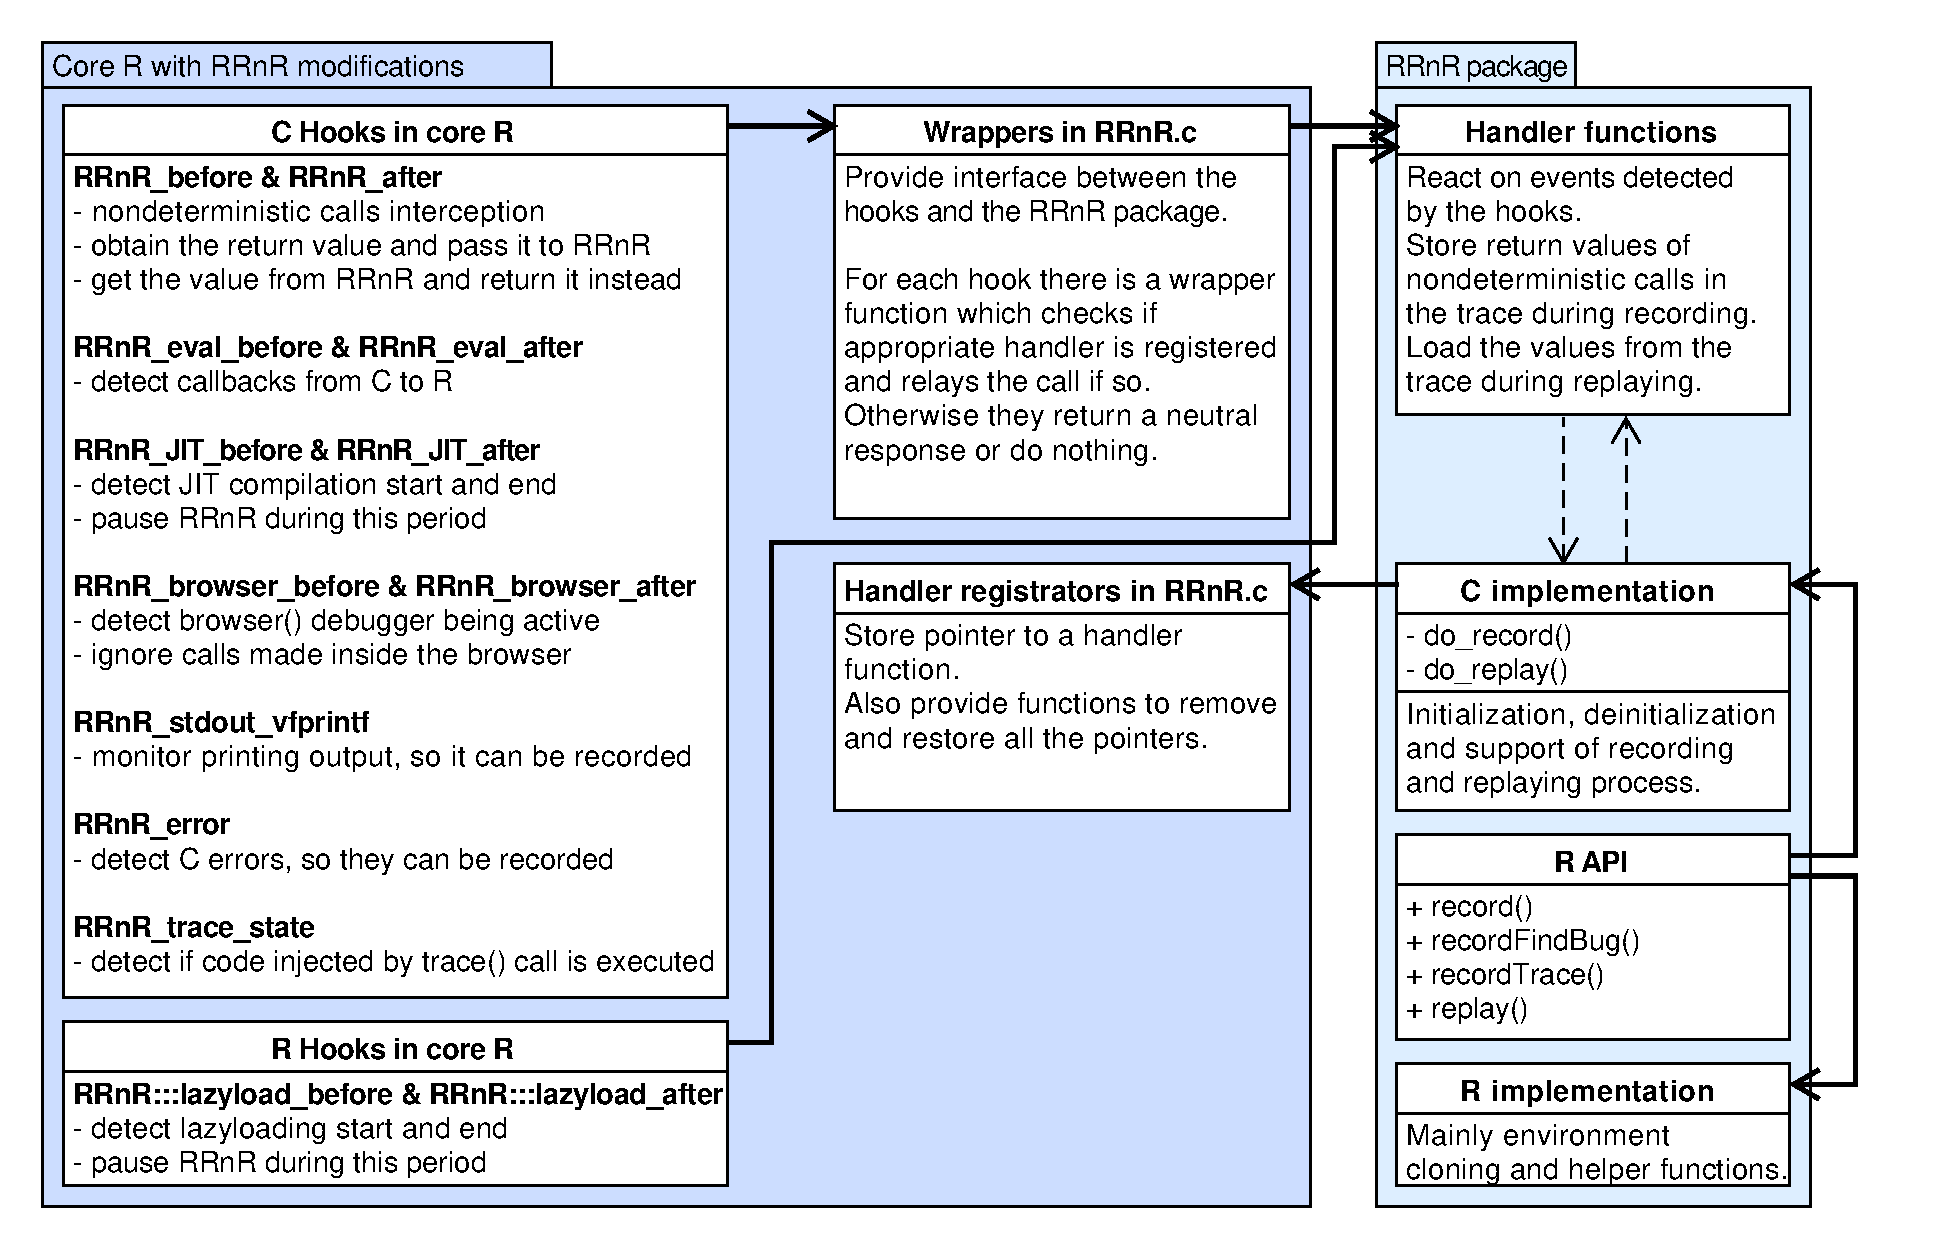
\includegraphics[width=1.0\textwidth]{img/incorporation_into_r2}
			\caption{Overview of the project architecture}\label{fig:incorporation_into_r2}
		\end{figure}
		
		It is also important to decide where the hooks capturing non-deterministic calls should be placed. After careful consideration of all possible approaches to the problem, focusing on the R's bytecode interpreter seems as the best solution. The \emph{compiler} package is among the base packages since version 2.13.0~\cite{r_compiler_included} and the JIT has been enabled by default since version 3.4.0~\cite{r_compiler_enabled}. Therefore it is almost obligatory to implement a solution with the ability to capture calls in the bytecode. As for capturing calls in the AST interpreter, it may seem like just a \qt{nice-to-have} feature as the percentage of such calls is negligible. However, as described further, there are some situations where R falls back to the AST interpreter and other implementation details which make it necessary to capture at least some of the non-bytecode calls as well.\par
	
		\subsection{Capturing non-determinism}
		Non-determinism cannot appear inside a plain R code because it is always based on some sort of a non-deterministic input and all I/O communication in R (e.g. generating a random number, reading a file or communicating over the Internet) happens either in internal C code or in external code written in Fortran or in any C-compatible language. There is no other way that would allow R code to interact with external resources. The bridge between the always deterministic R code and the possibly non-deterministic C/Fortran code is very narrow and therefore it is the perfect place for capturing the communication travelling through it.\par
		
		There is always a possibility that an external function non-deterministically changes the state of the R interpreter. However, such behaviour is generally undetectable as the external function can theoretically do anything from calling a simple R function to randomly overwriting memory of the process. To capture this, some external tool like the Mozilla's rr would have to be used together with RRnR but that is an extreme measure beyond the reach of this thesis.\par
		
		With this in mind it is possible to describe the bare minimum of how the capturing works. RRnR gets notified by a hook in the core R every time there happens a call of a non-deterministic C/Fortran function. It lets the function to execute and then stores the returned value into a data structure called \emph{trace}.\par
		
		Later during replaying RRnR again gets notified when there is a non-deterministic function being called but instead of executing the function it just returns the original value from the trace which was stored during the recording phase. Because the replay is deterministic it can be assumed that the contents of the trace are always delivered in the correct order corresponding with the functions being called.\par

		\subsection{Hooks}
		In order to achieve what has been described so far RRnR must be notified both \emph{before} and \emph{after} a non-deterministic call is executed. The \emph{before} is needed so that RRnR can control whether the call is allowed to be executed and the \emph{after} is needed to save the return value during recording and to load the return value stored in the trace during replaying.\par
		
		This is achieved by inserting small pieces of code (\emph{hooks}) into the core R around (before and after) important places. There is a limited amount of places where the hooks must be inserted, therefore RRnR can stay strongly separated from the core R as planned.\par
		
		The hooks are supposed to inform RRnR of being triggered by calling appropriate handler functions inside the RRnR package. However, it is not possible for a package function to be called directly from the core R as all packages are linked dynamically after startup. Instead, the package itself registers its handler functions first (before recording or replaying starts). The hooks then just call \emph{wrapper functions} in \emph{RRnR.c} which is a file added to the core R.\par
		
		The wrapper functions check whether there is an appropriate handler function registered and if so they relay the call to that handler function. Therefore RRnR package can stay separate from the core R and only if needed it can attach some of its functions as handlers.\par
		
		\begin{figure}[ht]\centering
			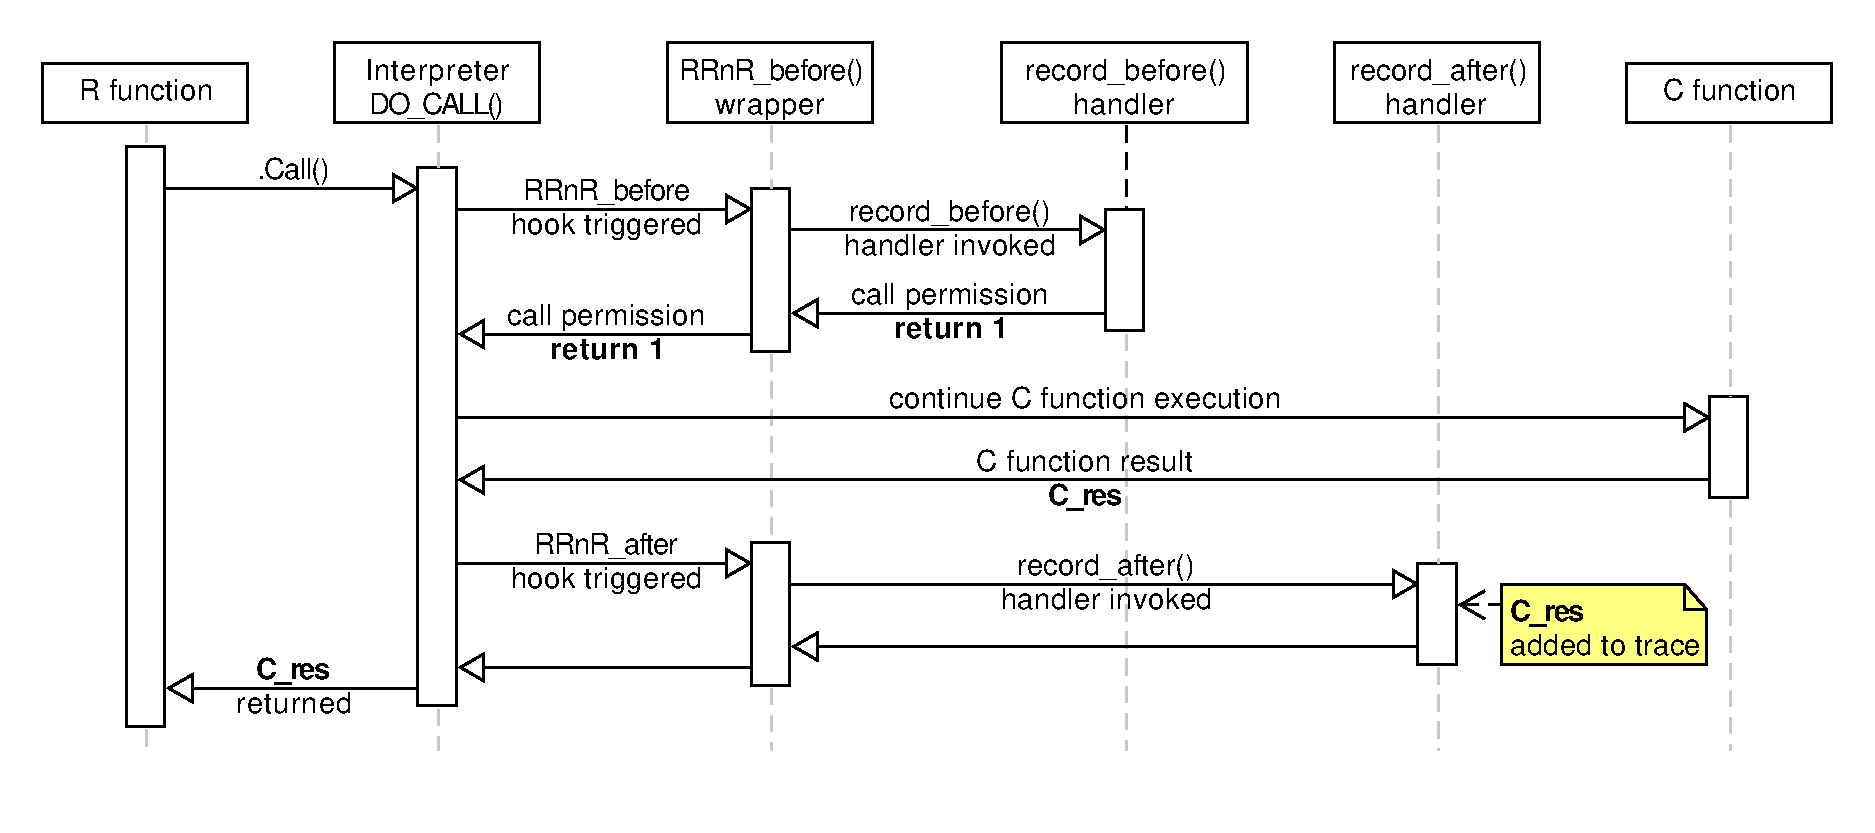
\includegraphics[width=1.0\textwidth]{img/call_capturing}
			\caption{Recording an external C function call}\label{fig:call_capturing}
		\end{figure}
		
		\begin{figure}[ht]\centering
			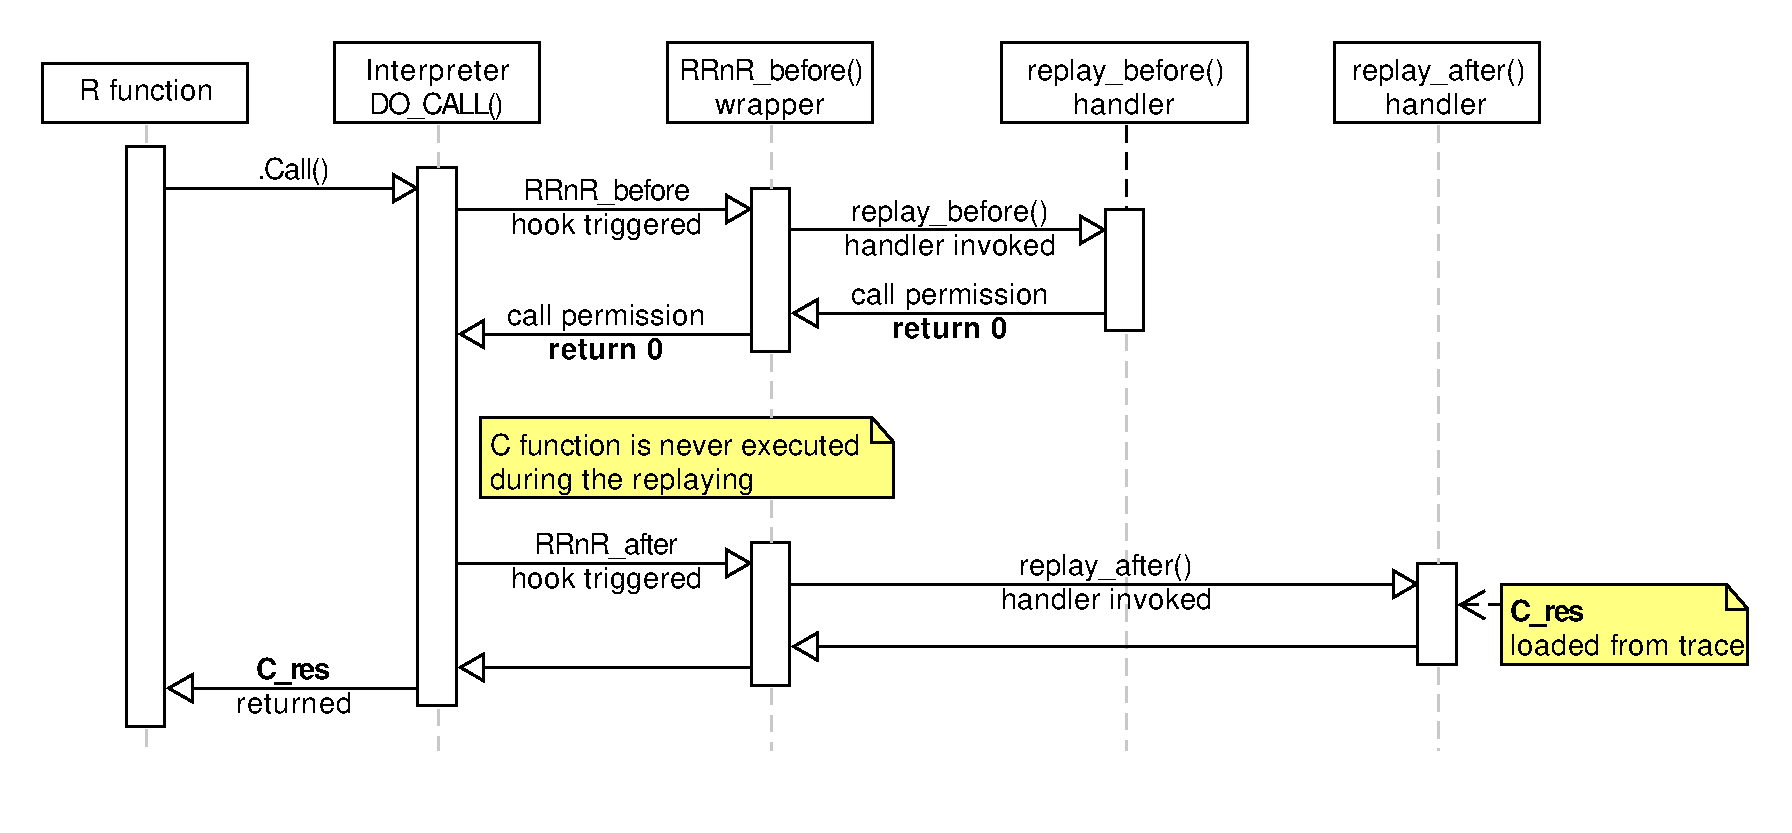
\includegraphics[width=1.0\textwidth]{img/call_capturing2}
			\caption{Replaying an external C function call}\label{fig:call_capturing2}
		\end{figure}
		
		\subsection{User interface}
		It is very important for RRnR to be user friendly, like the original R's debugger is. At least the basic functionality should be minimalistic and straightforward. If needed, it can be controlled in more detail by setting options. That is why there are just two main functions exposed to the user: \lstinline|record(expr, options)| and \lstinline|replay(rec)|.\par
		
		The \lstinline|record()| function takes an expression for which the evaluation should be recorded. The return value of this function is a list called \emph{replay structure} containing all the information necessary for the replay to work. It is possible to call \lstinline|record()| multiple times with different expressions, save the replay structures arbitrarily and then supply them to the \lstinline|replay()| function in any order. Once called, the \lstinline|replay()| function executes the expression contained in the replay structure in the exact same way it was recorded.\par
		
		User may store any number of replay structures though it should be noted that they can be quite large as they contain all input including contents of files loaded from disk. This behaviour and some others may be changed by setting an option.\par
		
		RRnR supports the standard debugging facilities in R hence the debugging process and its user interface are basically the same as during normal debugging session. Any \lstinline|browser()| calls inserted into the recorded function are invoked during replaying. Once the browser pauses the execution RRnR is also temporarily disabled which allows the user to execute any expression in the browser without affecting the replaying process.\par

	\section{RRnR core functionality}
	There are many corner cases which must be handled explicitly in order for RRnR to work but to make the text more understandable they are described separately in the section~\ref{dealing} while this section describes how the base concepts of RRnR work and how they are implemented.\par

		\subsection{Core R modifications}
		R version 3.4.3 has been used as the starting point and its source code has been modified in a few places. Firstly a new source file \emph{src/main/RRnR.c} has been added which contains handler registrators and wrapper functions. Secondly hooks have been inserted into a few files -- \emph{src/main/eval.c}, \emph{src/main/connections.c}, \emph{src/main/names.c}, \emph{src/main/main.c}, \emph{src/main/errors.c}, \emph{src/main/debug.c} and \emph{src/library/base/R/lazyload.R}. Finally there are two new header files -- \emph{src/include/RRnR.h} which provides function declarations for the hooks and \emph{include/RRnR.h} providing interface used by the RRnR package.\par
		
			\subsubsection{Handler registrators}
			The RRnR package uses the \emph{handler registrators} to register some of its functions as event handlers for certain hooks. The registrators are functions in the core R which take pointers to the handlers as their arguments. The pointers are stored in the core R and are later used by the wrapper functions to pass information from the hooks in the core R to the handlers in the package. The most important registrator is \lstinline|RRnR_register_handlers()| function which is used to register the main \emph{before} and \emph{after} handlers.\par
			
			Then there are also \lstinline|RRnR_get_|\lstinline|all_handlers()| and \lstinline|RRnR_restore_all_|\allowbreak\lstinline|handlers()| helper functions which can be used to make a backup of all pointers to the handlers and later restore them.\par
			
			Finally a \lstinline|RRnR_remove_|\allowbreak\lstinline|all_handlers()| function can be used to unregisters all the handlers at once. This mechanism also solves the problem of switching between states (record, replay and inactive) as there may be different handlers registered for recording and replaying and the handlers are completely removed when RRnR is inactive.\par
			
			\begin{figure}[ht]\centering
				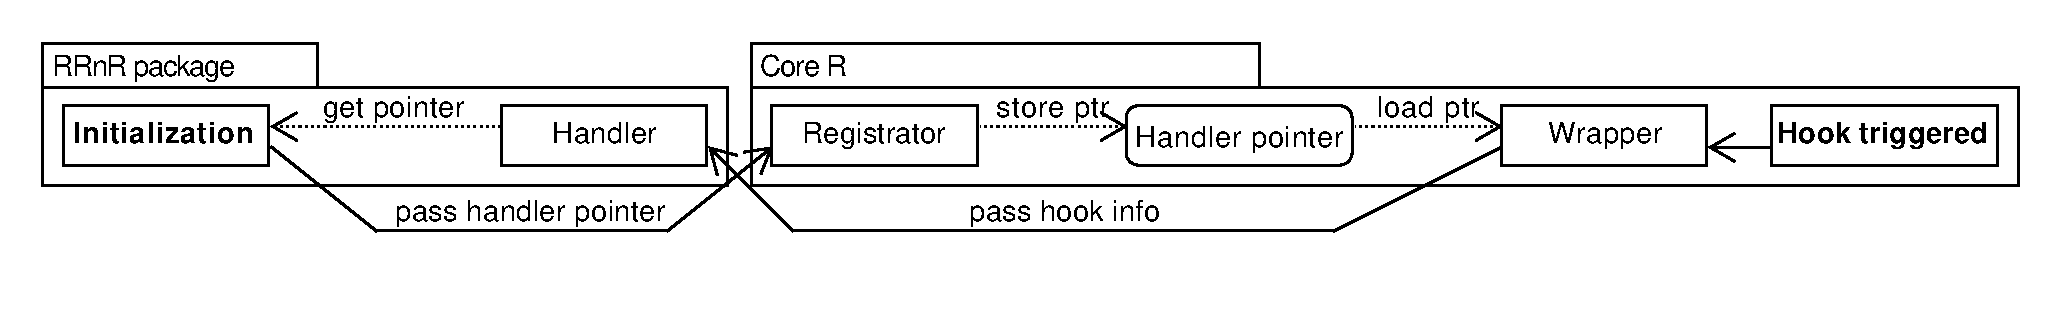
\includegraphics[width=1.0\textwidth]{img/registrators}
				\caption{Overview of handler registration and invocation process}\label{fig:registrators}
			\end{figure}
			
			\vspace{-12pt}
			\subsubsection{Wrapper functions}
			Wrapper functions are the means to connect the core R with the RRnR package. They are called by the hooks inside core R and then they pass the obtained information to RRnR via an event handler. There are two main wrapper functions needed in order to enable the basic record and replay functionality -- \lstinline|RRnR_before()| and \lstinline|RRnR_after()|. Their implementation is very simple as they only check if there is a corresponding event handler registered and if so they call it with the parameters acquired from the hooks.\par
			
			If there is no handler registered the wrapper functions return such value that causes R to work normally as if there were no hooks inserted. This means a value 1 for the \lstinline|RRnR_before()| and the original return value of the captured call for the \lstinline|RRnR_after()|.\par
			
\begin{lstlisting}[style=filestyle, language=C, caption={The \lstinline|RRnR_after()| wrapper function}]
SEXP RRnR_after(SEXP call, SEXP op, SEXP args, SEXP rho, int call_type, SEXP val) {
	return RRnR_after_handler
		? RRnR_after_handler(call, op, args, rho, call_type, val)
		: val;
}
\end{lstlisting}
			
			\subsubsection{Basic hooks}
			In order for the basic record and replay functionality to work there are only a few hooks needed in the core R code. It is sufficient to detect calls of the R internal functions in the bytecode interpreter which is located in the \emph{src/main/eval.c} file. The most important place is in a \lstinline|bcEval()| function, specifically in a part which handles a \lstinline|CALLBUILTIN| instruction.\par
			
			Calls to the \lstinline|RRnR_before()| and \lstinline|RRnR_after()| wrapper functions are inserted between the actual call of the builtin and the assignment of its return value. There are two places where the call can be made, one is used only in rare conditions with profiling enabled but the hook is inserted into both of them to increase robustness of the solution.\par
			
\begin{lstlisting}[style=filestyle, language=C, caption={The \emph{CALLBUILTIN} instruction hook}]
value = RRnR_after(call, fun, args, rho, RRNR_BUILTIN,
	RRnR_before(call, fun, args, rho, RRNR_BUILTIN)
	? PRIMFUN(fun) (call, fun, args, rho)
	: R_NilValue);
\end{lstlisting}
			
			There is also a \lstinline|CALLSPECIAL| instruction which calls special functions, but because there are no special functions which could potentially be non-deterministic it is safe to ignore this instruction.\par
			
			Furthermore there is a generic \lstinline|CALL| instruction which may be used for calling either builtins, specials or classic closures. One of the usages of the \lstinline|CALL| instruction is for calling functions with variable number of arguments. It is important to insert the hooks in this place as well in order to capture calls of these functions. The code is the same as for the \lstinline|CALLBUILTIN| instruction.\par
			
			Then there is a \lstinline|DOTCALL| instruction which is used just for \lstinline|.Call()| R function. As calling foreign functions is a typical source of non-determinism it is necessary to insert a hook there as well. Similarly to the \lstinline|CALLBUILTIN| instruction there are two code paths which may be used to execute the call and therefore both must be treated by inserting a hook.\par
		
		\subsection{RRnR package}
		As already mentioned, the majority of RRnR is implemented in an R base package. Base packages differ from standard packages mainly in the fact that they are a native part of R, meaning they are \qt{preinstalled}. There are also some minor differences in the implementation details regarding the way C functions are exposed to R. Base packages use the most verbose way of exposing functions by registering the native routines using the \lstinline|R_registerRoutines()| function. But other than that the structure of a base package is the same as any standard R package.\par
		
		The RRnR package is located in \emph{src/library/RRnR} folder. Inside there is a \emph{src} directory containing all the C code, \emph{R} directory containing all the R code, \emph{DESCRIPTION} and \emph{NAMESPACE} files. On top of that there are \emph{tests} and \emph{benchmarks} folders which contain code used for testing RRnR. The \emph{tests} folder contains unit tests runnable by \emph{testthat} tool (more in~\ref{testing}) whereas the \emph{benchmarks} folder contains a benchmarking tool and a set of benchmarks to measure the speed impact of using RRnR.\par
		
		There are two lines in the \emph{NAMESPACE} file which control the way the package functions are exposed to R. The first line says that all C functions can be called from R with a \emph{C\_} prefix. The second line lists all the functions which are exported to the global namespace once the package is loaded -- \lstinline|record()|, \lstinline|replay()|, \lstinline|recordTrace()| and \lstinline|recordFindBug()|.
		
			\subsubsection{Recording phase}
			The recording phase starts when a user calls the \lstinline|record()| function in R. It takes two arguments -- the expression that is to be recorded and an optional list with options controlling the behaviour of RRnR. The R function parses the options and then passes all necessary information to the C part of the package, specifically to the C \lstinline|do_record()| function. This function mainly initializes the trace and registers handler functions for the hooks.\par
			
			Then the expression is evaluated. During this time all the hooks are active and if a non-deterministic function is called the corresponding handler is notified and it adds the return value of the non-deterministic function to the trace.\par
			
			Once the expression evaluation is finished all the handlers are unregistered and the trace is returned back to the R \lstinline|record()| function wrapped inside the replay structure and from there it is simply returned to the user. The replay structure is a generic vector containing all the necessary data for the replaying to work, mainly the expression with its environment, the trace, the result of the evaluation and the list of options.\par

			\subsubsection{Parsing options}
			The options which may be passed to the \lstinline|record()| function are stored in a named list in a format of \emph{option\_name = option\_value}. The option list passed by a user is merged with a default option list. It is ensured that all options which are not set by the user are initialized to a default value and that all additional options in the user's list which are not known by RRnR are ignored.\par
			
			The merged options are then sent to the C \lstinline|do_record()| function where they are parsed and their values are stored in a global structure called \lstinline|RRnR_|\allowbreak\lstinline|options|. In there the individual options can be accessed from any C function of the RRnR package.\par
			
\begin{lstlisting}[style=filestyle, language=C, caption={Example of option parsing in C}]
int allow_gr = asLogical(getListElement(options, "allow_graphs"));
if(allow_gr == 0 || allow_gr == 1)
	RRnR_options.allow_graphs = allow_gr;
\end{lstlisting}
			
			\subsubsection{Passing the expression from R to C}
			The main purpose of the \lstinline|record()| function is to pass the expression, which a user wants to record, to the C part. This must be done in a way that does not cause the expression to be accidentally evaluated because RRnR is not yet prepared for recording at this point.\par
			
			All function arguments in R are passed as promises without being evaluated so it should be theoretically possible to just pass it along, however the \lstinline|.Call()| function, which is used to call the C function, always evaluates the arguments before passing them to C. The expression must be converted to an expression object of type \lstinline|EXPRSXP| instead, which is basically an AST representation of the expression. In this form it can be safely passed without evaluation.\par
			
			Besides the expression itself there is one more piece of information necessary for it to get evaluated in the C code. The \lstinline|eval()| function expects an environment as a second argument. In this case it should be the \emph{parent frame environment} inside which the R \lstinline|record()| function was called and in which the user expects the expression to be evaluated. The parent frame and the expression object can be obtained by two simple lines of code.\par
			
\begin{lstlisting}[style=filestyle, caption={Obtaining the expression and the environment}]
expr <- as.expression(substitute(expr))
env <- parent.frame()
\end{lstlisting}
			
			\subsubsection{Trace allocation and manipulation}
			The trace is initialized as an R list object, which in C is called a generic vector (\lstinline|VECSXP|). It is supposed to be filled with return values of the recorded functions, therefore it is important that it can contain objects of different data types. Because it is stored in a global variable it cannot be protected against deletion by the \lstinline|PROTECT()| macro. It must be registered as an exception in the garbage collector via the \lstinline|R_PreserveObject()| function instead.\par
			
\begin{lstlisting}[style=filestyle, language=C, caption={Initialization of the trace object}]
trace_sz = 16;
trace_cnt = 0;
R_PreserveObject(trace = allocVector(VECSXP, trace_sz));
\end{lstlisting}
			
			During recording the values are stored in the trace using \lstinline|add_to_trace()| helper function. As the trace is dynamically allocated it is necessary to increase its size when needed. There is a function in the R's C API which can be used to resize and reallocate a vector but it is important to keep in mind that the pointer to the vector changes in the process and therefore the object must be re-protected.\par
			
\begin{lstlisting}[style=filestyle, language=C, caption={Trace resizing in the \lstinline|add_to_trace()| function}, float, floatplacement=H]
if(trace_cnt >= trace_sz) {
	SEXP tmp;
	trace_sz *= 2;
	R_PreserveObject(tmp = lengthgets(trace, trace_sz));
	R_ReleaseObject(trace);
	trace = tmp;
}
\end{lstlisting}
			
			\subsubsection{Event handlers for recording}
			There are different handler implementations for the recording and the replaying phases. The recording version of the \emph{before} handler is very simple and always returns 1, which permits the call, because during recording the return value of the call must be stored in the trace.\par
			
			The record implementation of the \emph{after} handler must decide whether the call needs to be recorded or whether it is certainly deterministic and can be ignored. This detection is factored out in a separate function which is called \lstinline|detect_flags()|. If the call is marked as \lstinline|SHOULD_BE_HANDLED| then its return value is added to the trace using the \lstinline|add_to_trace()| function.\par
			
\begin{lstlisting}[style=filestyle, language=C, caption={Excerpt from the \lstinline|detect_flags()| function}]
int flags = 0;
...
if(is_device_opening_call(call, env))
	flags = SHOULD_BE_HANDLED | IS_DEVICE_OPENING;
else if(should_handle_call(call, args, env))
	flags = SHOULD_BE_HANDLED | CAN_PRODUCE_CALLBACK;
return flags;
\end{lstlisting}
			
			The \lstinline|detect_flags()| helper function uses all available information gathered by the hook to detect the properties of the function call and returns them in an easy-to-use format for further processing by the event handler. The result is returned in a form of a bitset of flags. Mainly the function detects whether a call should be recorded by setting the \lstinline|SHOULD_BE_HANDLED| flag. On top of that it divides calls into several categories which enables some special treatment in the handler.\par
			
			The detection is mostly based on the name of the called function. The name is obtained in a form of a symbol object which is an unique identifier and it is guaranteed that every time a certain function is called its symbol is the same object. Thus it can be simply and, what is more important, quickly compared with other symbols just by comparing their pointers. For each category of functions that the \lstinline|detect_flags()| function is supposed to identify there is an array of their symbols created. When a function call is to be categorized its symbol is simply compared with other symbols in the arrays.\par
			
\begin{lstlisting}[style=filestyle, language=C, caption={Detection of presence of a function symbol in the symbol database}]
if(!symbols_init) init_symbols();
SEXP func_symbol = CAR(call);
for(i = 0; i < num_to_handle; i++)
	if(symbols_to_handle[i] == func_symbol) return 1;
return 0;
\end{lstlisting}
			
			It is not necessary to compare symbols of primitive functions against the database because no primitive functions are considered non-deterministic. Therefore the processing of primitives is made much faster by using an \qt{early-out} condition first. Primitive function can be recognized by a \lstinline|PRIMINTERNAL()| macro.\par
			
			\subsubsection{Replaying phase}
			The \lstinline|replay()| function takes just a single parameter -- the replay structure created earlier by the \lstinline|record()| function. The replay structure is passed to the C \lstinline|do_replay()| function which unpacks all necessary information from it. Replaying versions of event handlers are registered and then the expression contained in the replay structure is evaluated.\par
			
			Once a possibly non-deterministic function call is detected by a hook it is processed by the handlers. Non-deterministic functions are not called, their return value is loaded from the trace instead. Once the expression evaluation is finished, all the handlers are unregistered and the control is returned back to the user.\par
			
\begin{lstlisting}[style=filestyle, language=C, caption={Replay structure unpacking example}]
if(TYPEOF(replay_struct) != VECSXP)
	error("replay structure must be a generic vector");
if(LENGTH(replay_struct) != 7)
	error("replay structure should have exactly seven elements");
SEXP expr = VECTOR_ELT(replay_struct, 0);
if(TYPEOF(expr) != EXPRSXP)
	error("expression must be an expression vector");
if(LENGTH(expr) != 1)
	error("exactly one expression expected");
\end{lstlisting}
			
			\subsubsection{Reading values from the trace}
			The replaying version of the \emph{after} handler calls the \lstinline|detect_flags()| function. When the \lstinline|SHOULD_BE_HANDLED| flag is set it means that the current call is not permitted to be executed and its return value should be read from the trace instead.\par

			A variable called \lstinline|trace_pos| is used to store the current position in the trace. In the beginning it is set to zero and with every replayed call its value is increased. The replay is supposed be deterministic and therefore it is expected that the number of replayed calls is exactly the same as the number of recorded calls and that the currently used trace value corresponds with the currently replayed call.\par
			
			If the \lstinline|trace_pos| variable points behind the end of the trace it is a sign that something went wrong and therefore the execution must be terminated by sending an error via the \lstinline|stop()| API function.\par
			
\begin{lstlisting}[style=filestyle, language=C, caption={Trace reading functions \lstinline|peek_trace()| and \lstinline|read_trace()|}]
SEXP peek_trace() {
	if(trace_pos < trace_cnt) return VECTOR_ELT(trace, trace_pos);
	else error("no more recorded calls");
}
SEXP read_trace() {
	SEXP ret = peek_trace();
	trace_pos++;
	return ret;
}
\end{lstlisting}
		
	\section{Dealing with corner cases}\label{dealing}
	The implementation as described in the \emph{RRnR core functionality} section is usable only for the simplest cases. There are many corner cases which have to be handled separately. Similarly to Mozilla rr RRnR is not trying to create an ultimate solution for every possible scenario. But by focusing on the most common problems, which are described in this section, RRnR aims to cover the largest possible portion of use cases while keeping the scale of the project manageable.\par
	
	The most important problems to deal with are detection and replaying of \emph{callbacks} from C to R, restoring the same environment state before each replaying by \emph{environment cloning}, avoiding invalid environment references by \emph{environment in-trace replacement}, monitoring \emph{prints} in order to replay them properly, properly replaying \emph{graphics} output, making sure that \emph{debugging} works, ignoring one-time code evaluation like \emph{JIT} compilation and \emph{lazy loading}, properly replaying \emph{errors} and handling \emph{invisible returns}.\par
	
		\subsection{Callbacks}
		When an external function call is replayed its return value is read from the trace but the call itself is never executed again as it may contain some non-deterministic code. A problem occurs when the external function uses the \lstinline|eval()| function to call back to R. If the external function is not replayed then neither is the R code which is not optimal. Firstly the user may want to debug the R code and in order to be able to do that the code must be executed. And secondly there might be possible side effects caused by the R code which should be replicated during the replaying in order to maintain determinism.\par
		
\begin{lstlisting}[style=filestyle, caption={Simple example of the callback problem}]
rec <- record(x <- .Call(C_func)) # C ret value added to the trace
x <- replay(rec)                  # value loaded from the trace
------------------------------------------------------------------
// C:
  SEXP C_func() {                    // never replayed
    return eval("R_func()");
  }
# R:
  R_func <- function() {             # never replayed (PROBLEM)
    runif(1)
  }
\end{lstlisting}

		To solve this problem it is necessary to detect the callbacks when recording and store all the necessary information in the trace as shown in the diagram~\ref{fig:callbacks}. Then in the replaying phase the information is read from the trace and the callbacks are replayed as shown in the diagram~\ref{fig:callbacks2}. This way the external function is still not replayed but the eval'd R code is executed the same way as it was during recording. The process works recursively so when the R code makes other non-deterministic calls they are also recorded and not replayed. \par
		
		\vspace{-10pt}
		\begin{figure}[ht]\centering
			\setlength{\abovecaptionskip}{-15pt}
			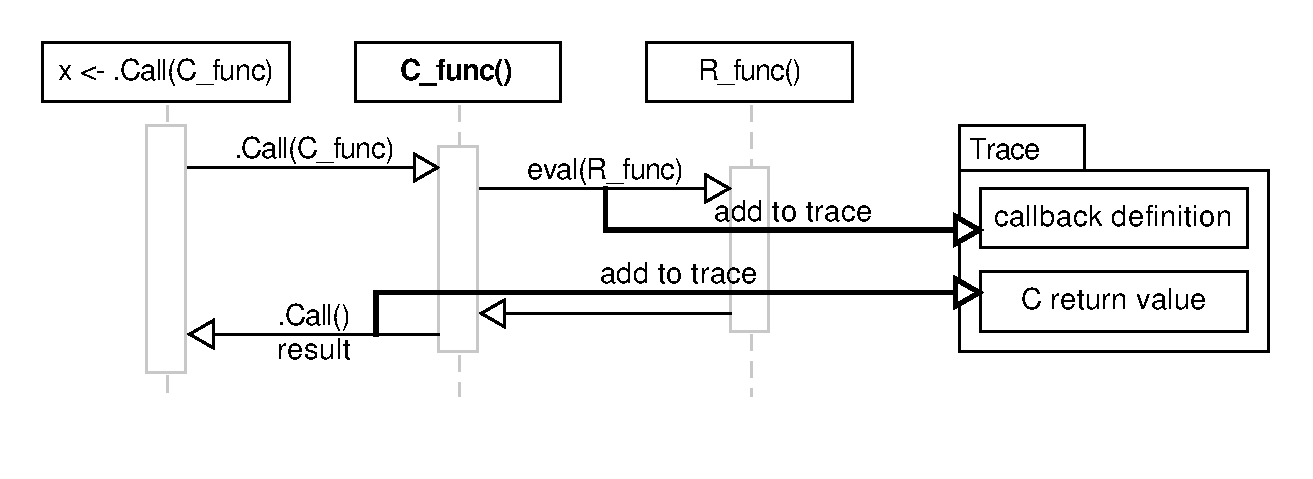
\includegraphics[width=1.0\textwidth]{img/callbacks}
			\caption{Recording the example callback}\label{fig:callbacks}
		\end{figure}
		
		\vspace{-10pt}
		\begin{figure}[ht]\centering
			\setlength{\abovecaptionskip}{-15pt}
			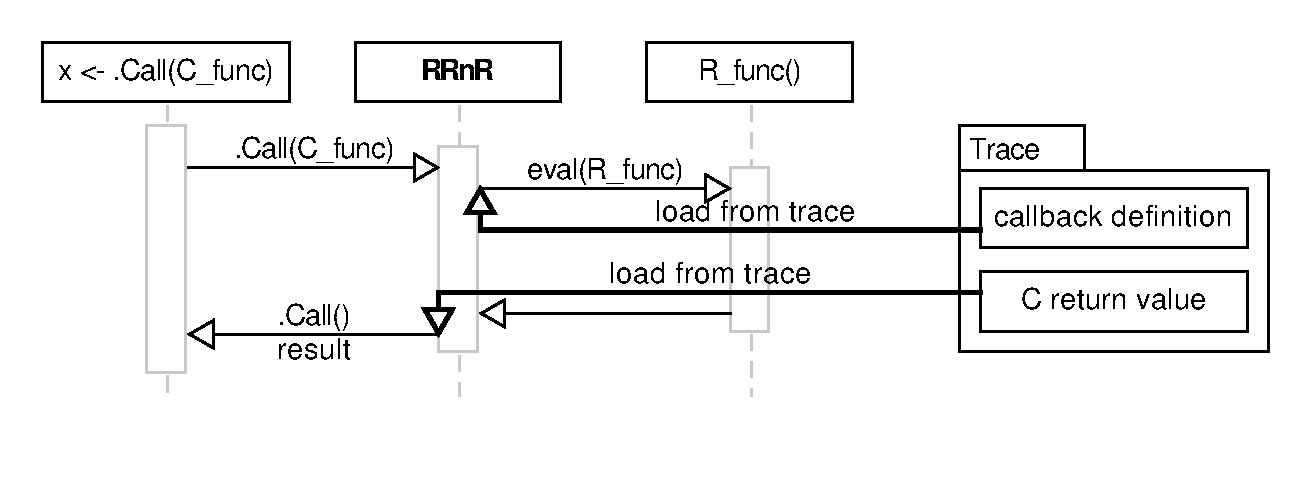
\includegraphics[width=1.0\textwidth]{img/callbacks2}
			\caption{Replaying the example callback}\label{fig:callbacks2}
		\end{figure}
		\FloatBarrier
		
			\subsubsection{Callback detection}\label{eval_handler}
			The only way for an external function to make a callback is by using the \lstinline|eval()| function, therefore the detection is implemented by inserting two hooks in there, one hook is inserted at the beginning (\emph{eval\_before}) and one at the end (\emph{eval\_after}). The function is located in the \emph{src/main/eval.c} file.\par
			
			During recording the \emph{eval\_before} hook is triggered when the \lstinline|eval()| function is called. The arguments of the call (an expression and an environment) are stored in the trace with a special attribute marking them as \emph{\_RRnR\_callback}.\par
			
			However, not all invocations of the \lstinline|eval()| function are caused by a callback. In fact this function is called quite often. That is why the \emph{eval\_before} and \emph{eval\_after} handlers are not permanently active. They are registered in the basic \emph{before} handler just before an external function call is made.\par
			
			An external function call is simply recognized in the \lstinline|detect_flags()| function which sets a \lstinline|CAN_PRODUCE_CALLBACK| flag for any of these functions: \lstinline|.Call()|, \lstinline|.Call.graphics()|, \lstinline|.C()|, \lstinline|.Fortran()|, \lstinline|.External()|, \lstinline|.External2()|,\\\lstinline|.External.graphics()|.\par
			
			It is important that only the first \lstinline|eval()| call triggers the \emph{eval\_before} hook. The other calls which might happen are irrelevant for the callback detection. Therefore the \emph{eval\_before} handler must be unregistered immediately after being called.\par
			
			However, it is important to detect when the first \lstinline|eval()| call ends and returns the control back to the external function, because then the \emph{eval\_before} handler must be registered again in order to catch any other callbacks. This is ensured by the \emph{eval\_after} hook.\par
			
			This means that the \emph{eval\_after} handler cannot be unregistered unlike the \emph{eval\_before} one. But it must be ensured that the \emph{eval\_after} hook is triggered only in the first \lstinline|eval()| call and not in the other ones invoked during the R expression evaluation.\par
			
			This is achieved by the \lstinline|hook_enabled| variable in the \lstinline|eval()| function. If the \emph{eval\_before} handler is registered than the variable is set to \lstinline|TRUE|, otherwise it is set to \lstinline|FALSE|. The \emph{eval\_after} hook is triggered only if the variable contains \lstinline|TRUE|. The presence of the \emph{eval\_before} handler is signalled by the return value of the \emph{eval\_before} wrapper function.\par
			
			There might be a situation where the callback recursively calls another external function which executes another callback. This situation is fully supported as the whole solution is stack based using the implicit call stack for all the information including the \lstinline|hook_enabled| variable.\par
			
			But it is important to note that the \emph{eval\_after} handler must never be unregistered, not even after an external call is finished, because of the possibility of it being called recursively.\par
			
			\begin{figure}[ht]\centering
				\setlength{\abovecaptionskip}{-10pt}
				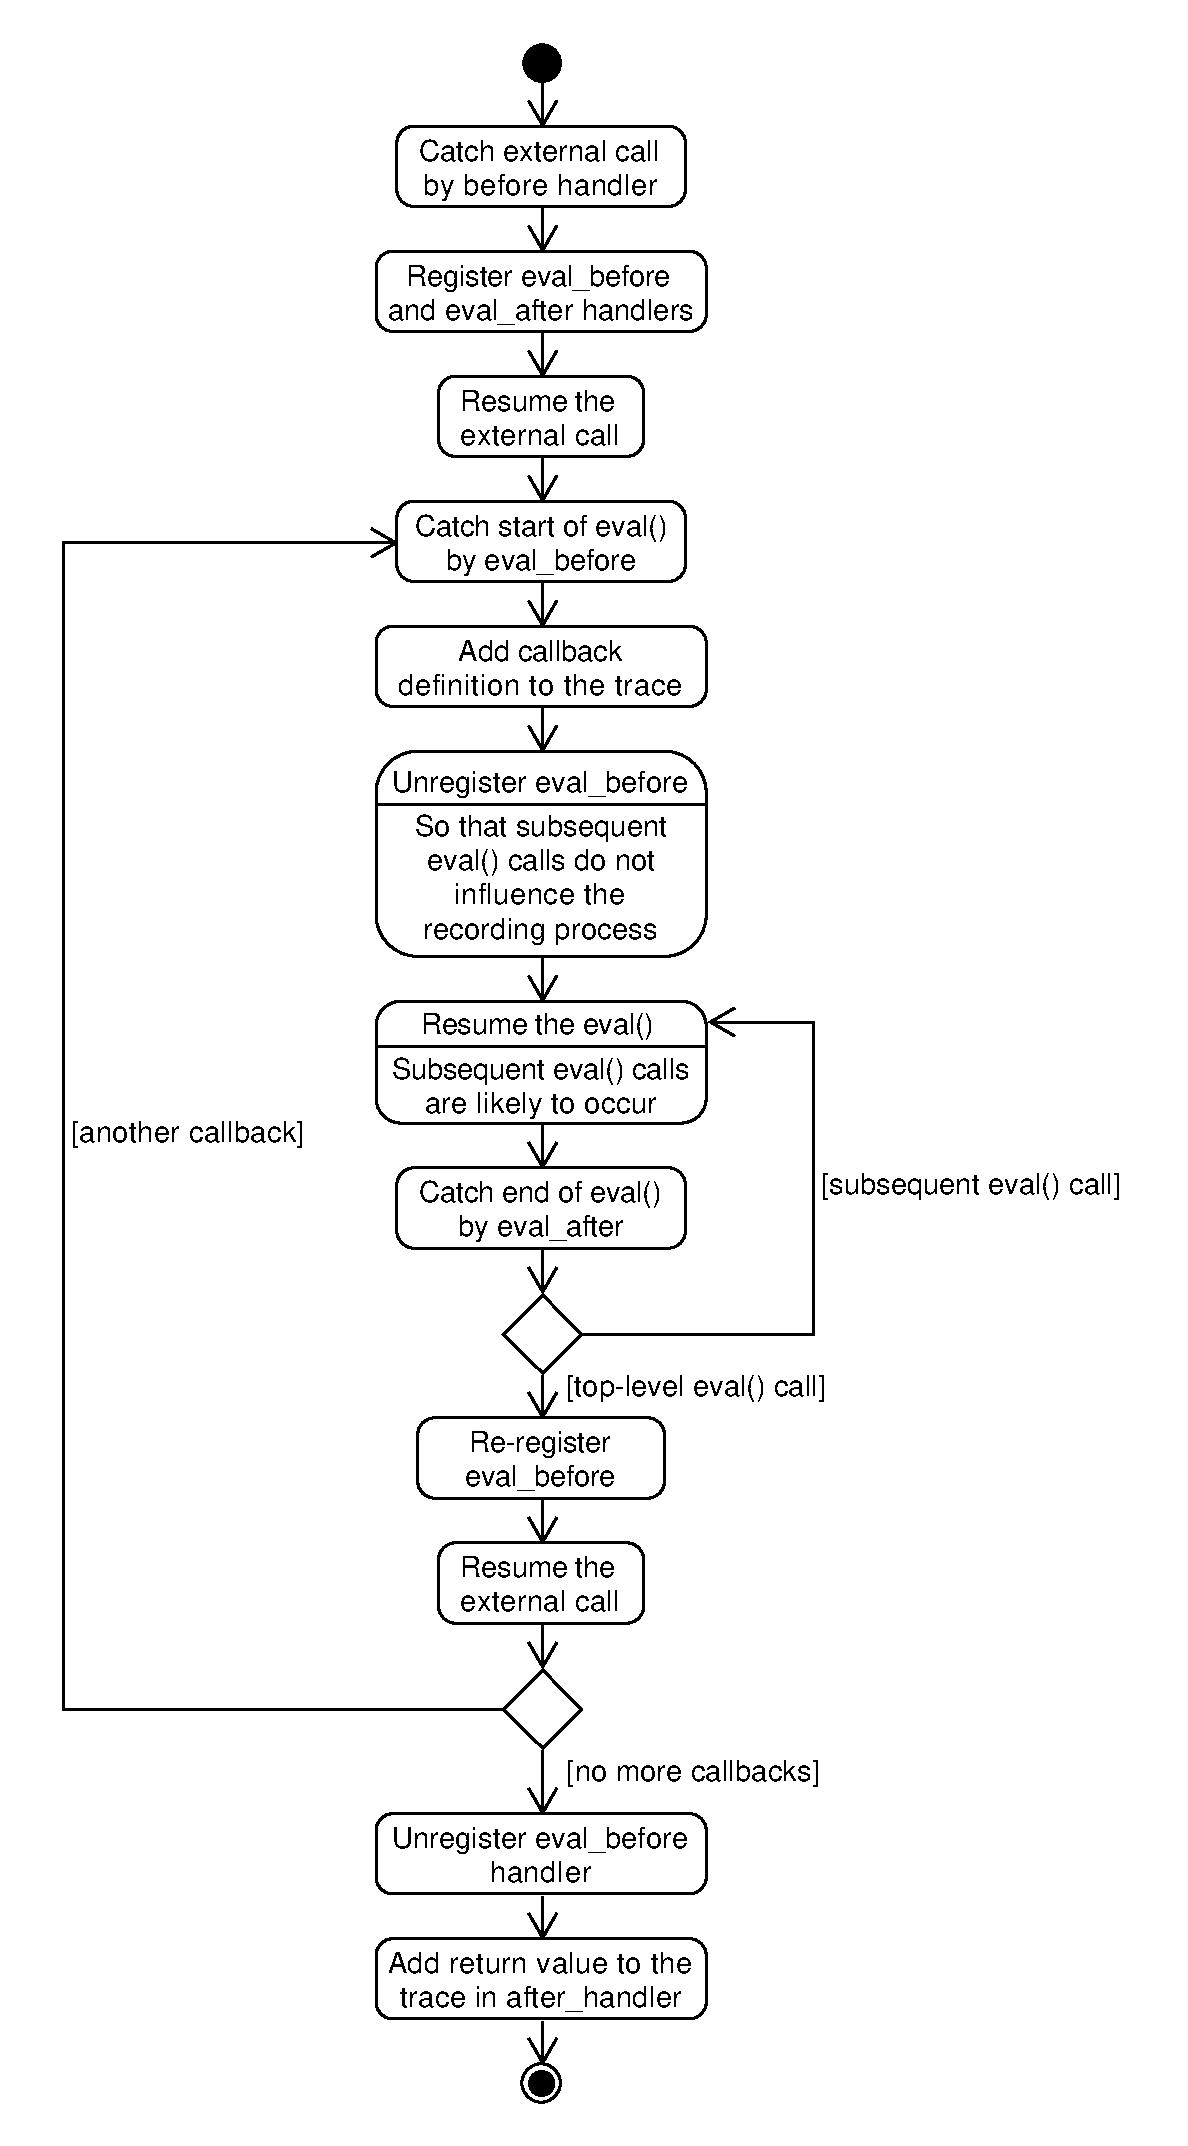
\includegraphics[width=0.9\textwidth]{img/callbacks3}
				\caption{Overview of the callback detection process}\label{fig:callbacks3}
			\end{figure}
			\FloatBarrier
			
			\subsubsection{Callback replaying}
			The replay functionality for the callbacks is entirely based on the contents of the trace. When a normal function call is replayed from the trace there is only the recorded return value at the current position in the trace. However, when there have been any callbacks then the trace also contains the parameters given to the \lstinline|eval()| function (an expression and an environment).\par
			
			During replaying all the callbacks happen in the exact same order as they happened during recording. Therefore it is sufficient to keep iterating through the trace while evaluating the callbacks until there is only the return value of the external function left. The callbacks can be identified by the \emph{\_RRnR\_callback} attribute. The evaluation of a callback is done simply by using the \lstinline|eval()| function with the loaded expression and environment.\par
			
\begin{lstlisting}[style=filestyle, language=C, caption={Iterating over the trace in the \emph{after} handler during replay}]
for(;;) {
	ret = PROTECT(read_trace());
	if(TYPEOF(ret) == VECSXP &&
	  getAttrib(ret, install("_RRnR_callback")) != R_NilValue) {
		SEXP call = VECTOR_ELT(ret, 0);
		SEXP env = VECTOR_ELT(ret, 1);
		eval(call, env);
		continue;
	}
	return ret;
}
\end{lstlisting}
			
			\subsubsection{Suppressors}
			The steps described above are applied only to \emph{external} function calls but in some situations it might happen that an R code is evaluated from a C function which is \emph{inside} the core R and is being recorded because of its non-determinism. One of such functions is \lstinline|print.function()| which uses \lstinline|eval()| to call \lstinline|as.character()| R function which is used to convert source reference of a function to character string. Such callbacks are deliberately ignored as they do not invoke any user code and have no side effects.\par
			
			However, it is important to ignore the entire execution of the callback code, not just the fact that there has been a callback. Otherwise the return values of some potential calls made by the code would be stored in the trace, but these values would never be retrieved from the trace in the replaying phase, because in this phase the callback code would be ignored, and that would result in a trace corruption.\par
			
			Therefore there are two special event handlers for the \emph{eval\_before} and \emph{eval\_after} hooks which are called the \emph{suppressors}. Their purpose is to temporarily suppress detection of all calls while a callback is being executed. They are registered in the standard \emph{before} handler for any call that is not explicitly allowed to have its callbacks captured. The implementation of the suppressors is very simple. The \emph{eval\_before} suppressor handler unregisters all handlers except the \emph{eval\_after} suppressor handler which is used to re-register the original handlers.\par
			
\begin{lstlisting}[style=filestyle, language=C, caption={Implementation of the suppressors}]
void * old_handlers_before_suppressor[7];
void eval_suppressor_before(SEXP call, SEXP env) {
	RRnR_remove_all_handlers(old_handlers_before_suppressor);
	RRnR_register_eval_handlers(NULL, eval_suppressor_after);
}
void eval_suppressor_after() {
	RRnR_restore_all_handlers(old_handlers_before_suppressor);
}
\end{lstlisting}

		\subsection{Environment cloning}
		Although R is strongly influenced by functional programming it definitely is not purely functional itself. Many functions in R have side effects and parent scopes are often modified using the \lstinline|<<-| operator. This can be a problem in the context of RRnR. If a function's output depends on a variable declared in its enclosing environment then the output is not guaranteed to be the same between individual replays of the function (as shown in the following example).\par
		
\begin{lstlisting}[style=filestyle, caption={Demonstration of manual environment modification problem}]
a <- 5
func <- function() print(a)
rec <- record(func())        # outputs 5
replay(rec)                  # outputs 5
a <- 6
replay(rec)                  # outputs 6 (should output 5)
\end{lstlisting}
		
		The first possible solution to this problem is very simple -- just pass the problem on to the user. It can be simply stated that the user is responsible for the consequences of all the changes in the environments he makes between recording and replaying.\par
		
		This is a valid solution for the example shown above but not so valid when the code being recorded is itself influencing the outer environment as shown in the example below. In this case the user would have to manually reset the changes before every replaying which is quite impractical as the user would have to keep track of all the changes that happen.\par
		
\begin{lstlisting}[style=filestyle, caption={Demonstration of inherent environment modification problem}]
a <- 5
func <- function() { print(a); a <<- a + 1; }
rec <- record(func())        # outputs 5
replay(rec)                  # outputs 6
replay(rec)                  # outputs 7
\end{lstlisting}
		
		Another possible solution leverages the already implemented recording system. If each read from an environment was recorded and its result stored in the trace then the real contents of the environments would not be relevant as the values would always be read from the trace. Therefore all changes made in the environments after the recording is done would not alter the execution of the code in the replaying mode.\par
		
		The biggest drawback of this solution is the performance and memory overhead as every single variable access would have to be recorded which makes the solution practically unusable.\par
		
		The solution which is actually used in RRnR is based on the first one but rather than forcing the user to reset the environments manually RRnR does it automatically. Before the recording begins all relevant environments are cloned and the clones are stored in the replay structure. Then before each replaying the content of the active environments is replaced by the content of the clones which effectively reverts it to the state before the recording.\par
		
		However, this introduces another problem which is visible after the first replaying. The environments are cloned \emph{before} the \lstinline|record()| function returns the replay structure. Therefore the replay structure is not contained in any of the cloned environments. When the active environments are replaced by the clones in the \lstinline|replay()| function the replay structure is removed which makes it impossible to do a second replaying as shown in the example below.\par
		
\begin{lstlisting}[style=filestyle, caption={Demonstration of environment replacement problem}]
a <- 5                 # env{a}
rec <- record(func())  # env{a}, clone <- env, env{a, rec}
replay(rec)            # env{a, rec}, env <- clone, env{a}
replay(rec)            # Error: object 'rec' not found
\end{lstlisting}
		
		This is solved by creating additional clones at the beginning of the \lstinline|replay()| function. Then at the end of the function the active environments are reverted to the original state using this clones.\par
		
		Finally there is one more problem to solve which happens when recording is done multiple times. After the first recording there is a replay structure stored in a variable. During the second recording this variable is cloned along with the current environment and stored in the new replay structure.\par
		
		When recording multiple times this creates a chain in which the newest replay structure contains all the previous ones. Because a replay structure might be quite big there is a potential memory depletion problem. Therefore when cloning before recording all replay structures are detected by a special attribute and ignored.\par
		
		The cloning is implemented entirely in the R part of the RRnR package as it is the most convenient way. The implementation is divided into several functions. There are two main functions, one is called \lstinline|clone_environments()| (creates the clones from the active environments) and the other one is \lstinline|replace_|\allowbreak\lstinline|environments()| (replaces the active environments by the clones). Both of them use a function called \lstinline|iterate_environments()| which iterates over all the active environments. This function gets a callback as an argument and calls the callback on each of the active environments it iterates over.\par
		
		Finally there are two functions called \lstinline|clone_environment()| and \lstinline|replace_|\allowbreak\lstinline|environment()| which perform the actual work (cloning or replacing) on a single environment.\par
		
		The \lstinline|clone_environments()| function supplies a callback to the \lstinline|iterate_|\allowbreak\lstinline|environments()| function. The callback calls the \lstinline|clone_environment()| function and stores the result in a list. The \lstinline|replace_environments()| function supplies a callback which retrieves a cloned environment from the list and passes it to the \lstinline|replace_environment()| function.\par
		
			\subsubsection{Iterating over the environments}
			The \lstinline|iterate_environments()| function iterates over environments on the search path starting from a given environment and ascending by using the \lstinline|parent.env()| built-in function until a target environment is reached. It is important to note how the environments are arranged which can be seen in the following picture.\par
			
			\begin{figure}[ht]\centering
				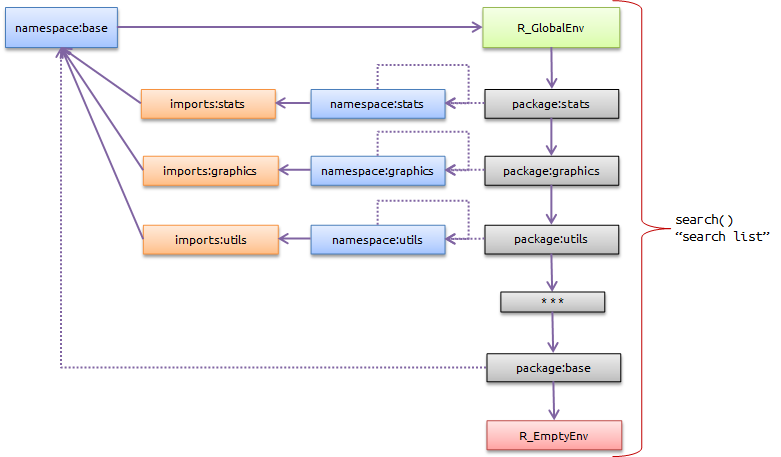
\includegraphics[width=1.0\textwidth]{img/environments}
				\caption{Arrangement of environments, taken from \cite{environments}}\label{fig:environments}
			\end{figure}
			
			Typically users are recording an expression defined either inside a package or in the global environment. In both cases there may be some local enclosing environments (not shown in the picture) which are then enclosed by either the namespace environment of the package or the global environment.\par
			
			In most cases the package environments, which are \qt{above} the global environment on the search path, are not changed between the record and replay phases and do not have to be cloned.\par
			
			However, in some rare cases it might be useful and that is why there is a \lstinline|full_clone| parameter (controlled by an option) which enables cloning of the package environments. But this process takes extra time.\par
			
			The namespace and imports environments cannot be cloned and are therefore skipped.\par
			
\begin{lstlisting}[style=filestyle, caption={The \lstinline|iterate_environments()| function}]
while(TRUE){ if(.Internal(isNamespaceEnv(env))) skip <- TRUE
             if(identical(env, .GlobalEnv)) skip <- FALSE
             if(identical(env, baseenv())) break()
             if(!skip) callback(env)
             if(!full_clone && identical(env, .GlobalEnv)) break()
             env <- parent.env(env) }
\end{lstlisting}
		
			\subsubsection{Cloning an environment}
			The \lstinline|clone_environment()| function creates a complete clone of a given environment. Environments can be locked against addition or removal of elements and individual elements can be locked against modification. In order to make a perfect clone it is necessary to properly set the locks in the clone.\par
		
\begin{lstlisting}[style=filestyle, caption={The \lstinline|clone_environment()| function}]
new_env <- new.env()
for(n in ls(envir=env, all.names=TRUE)) {
  obj <- get(n, envir=env)
  if(!skip_replay_structures ||
    !("RRnR_replay_structure" %in% names(attributes(obj))))
      assign(n, obj, envir=new_env)
}
parent.env(new_env) <- parent.env(env)

for(n in ls(envir=env, all.names=TRUE))
  if(bindingIsLocked(n, env)) lockBinding(n, new_env)
if(environmentIsLocked(env)) lockEnvironment(new_env, FALSE)
\end{lstlisting}
		
			\vspace{-15pt}
			\subsubsection{Replacing an environment}
			The \lstinline|replace_environment()| function replaces all contents of a given environment by contents of another given environment. This is done by first removing contents of the destination environment. To do that it is important to unlock the elements and the environment itself.\par
			
			R, however, does not support unlocking an environment from user-level code, therefore the unlocking is done by a custom C function which uses internal macros.\par
			
\begin{lstlisting}[style=filestyle, language=C, caption={Custom environment unlocking function}]
#define FRAME_LOCK_MASK (1<<14)
SEXP do_unlock_env(SEXP env) {
	SET_ENVFLAGS(env, ENVFLAGS(env) & (~FRAME_LOCK_MASK));
	return R_NilValue; }
\end{lstlisting}
			
			After that the contents of the source environment are copied into the destination environment and the elements are locked if needed as is the environment itself. The two \lstinline|force()| function calls at the beginning are used to force the evaluation of the function's parameters as their definition may be dependent on the contents of the destination environment. If the promises were not forced they would be evaluated when first used which might be after their values have been replaced in the destination environment.\par
		
\begin{lstlisting}[style=filestyle, caption={The \lstinline|replace_environment()| function}]
force(src_env)
force(dst_env)
.Call(C_do_unlock_env, dst_env)
for(n in ls(envir=dst_env, all.names=TRUE)) {
	unlockBinding(n, dst_env)
	rm(list=n, envir=dst_env)
}
for(n in ls(envir=src_env, all.names=TRUE)) {
	assign(n, get(n, envir=src_env), envir=dst_env)
	if(bindingIsLocked(n, src_env)) lockBinding(n, dst_env)
}
if(environmentIsLocked(src_env)) lockEnvironment(dst_env, FALSE)
\end{lstlisting}
		
		\subsection{Environment in-trace replacement}
		Environments in R have a special property. Unlike most other objects they use \emph{reference semantics}. This means that when an environment is assigned to a variable it is not copied but only a new \emph{reference} to it is created and stored in the variable. Therefore when the same environment is assigned to two variables \lstinline|A| and \lstinline|B| and a symbol is inserted into it using the first variable \lstinline|A$x <- 5| then the same symbol is also visible while accessing the environment using the second variable \lstinline|B$x|.\par
		
\begin{lstlisting}[style=filestyle, caption={Example code where reference semantics cause the problem}]
# R:
env <- environment()
rnd <- runif(1)
env <- .Call(C_return, env)
useEnv(env)
// C:
SEXP C_return(SEXP e) { return e; }
\end{lstlisting}

		Regarding RRnR this poses a serious problem in some cases which is best shown on an example code above. When using RRnR as described so far to record and replay the example code the trace contains only the result of the C call which is the return value of the \lstinline|environment()| call.\par
		
		The problem is that the environment reference returned by the function is different in each run because the environments are newly allocated every time. Therefore in the replaying run the current environment is different than in the recording run. But the value which is stored in the trace remains the same hence the return value of the \lstinline|.Call()| is also the same. But then the \lstinline|useEnv()| function is called with an environment reference that is no longer valid in the current run which will cause a completely different (most likely erroneous) behaviour.\par
		
		In the example the the C function is supposed to return the value of the current environment which is \lstinline|0x123| but the original \lstinline|0xABC| is loaded from the trace and returned instead, causing the \lstinline|useEnv()| function to fail.\par
		
		\begin{figure}[ht]\centering
			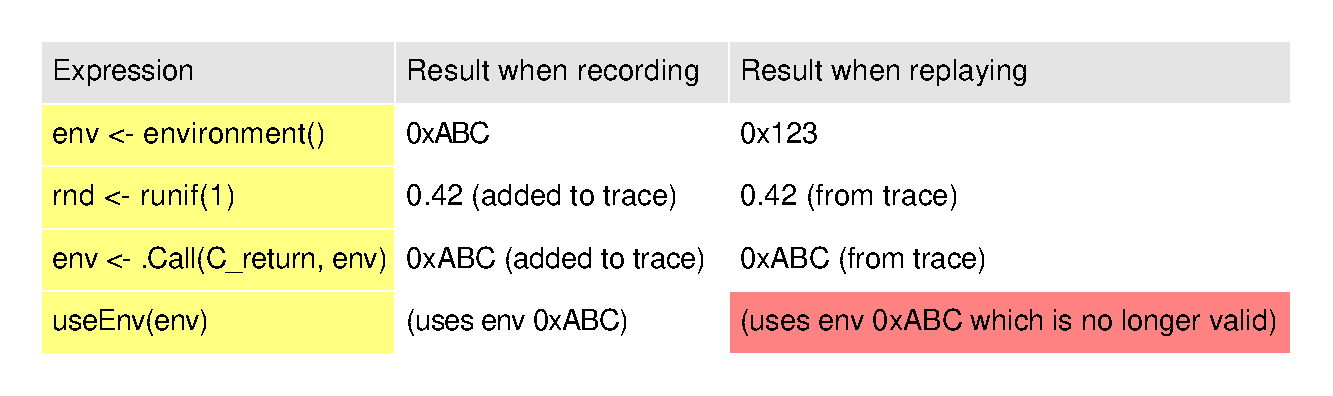
\includegraphics[width=1.0\textwidth]{img/env_replace}
			\caption{Overview of the situation \emph{without} environment replacement}\label{fig:env_replace}
		\end{figure}
		
		\begin{figure}[ht]\centering
			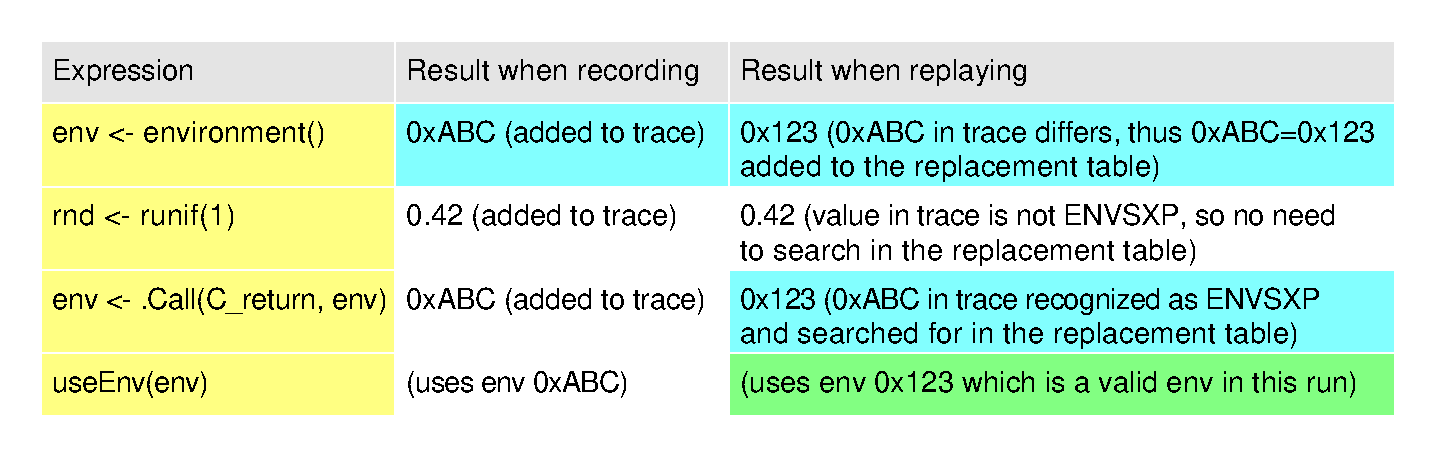
\includegraphics[width=1.0\textwidth]{img/env_replace2}
			\caption{Overview of the situation \emph{with} environment replacement}\label{fig:env_replace2}
		\end{figure}
		
		This problem is solved by recording return values of all functions which generate a reference to an environment, they are further referred to as the \emph{environment generators}. Examples of such functions are \lstinline|new.env()|, \lstinline|environment()| or \lstinline|parent.frame()|. Their return values are also stored in the trace. Then during replaying when a generator is called its new return value is compared to the original one. If it differs then during all further uses of the original value the new value must be used instead.\par
		
		Because of that there is a replacement table created which maps all the original values to the new ones. Every time an environment reference is being loaded from the trace it is first looked up in the table and the correct value is returned. The replacement is search for only if the value being loaded from the trace is of the type \lstinline|ENVSXP|, loads of other values are performed immediately without any modifications.\par
		
		In the example code, when the \lstinline|environment()| function is called during replaying, the \lstinline|0xABC| value is loaded from the trace and it is compared to the new return value \lstinline|0x123|. Because they are different a new replacement record is added to the replacement table. Then the replay continues normally and when the \lstinline|.Call()| is replayed the \lstinline|0xABC| value in the trace is recognized as an environment reference, and therefore the correct value is looked up in the table.\par
		
		The replacement table is stored in a global variable similarly how the trace is. The only difference is that the replacement table is supposed to store keys and values and that is why it is implemented as two separate generic vectors. The first one stores the keys and the second one the corresponding values. Both are initialized at the beginning of the \lstinline|do_replay()| function and deinitialized at the end.\par
		
		The addition of the replacement records is managed by a function called \lstinline|add_env_replacement()| which is very similar to the \lstinline|add_to_trace()| function including the resizing code which dynamically doubles the size of the vectors if needed. And then there is a \lstinline|replace_env()| function which takes an environment, searches through the keys vector for the given environment and returns the corresponding value if found. Otherwise it returns the argument itself.\par
		
		The \lstinline|replace_env()| function is used at two places. The first one is in the callback replaying code where the environment passed to the \lstinline|eval()| function must be replaced. And the second one is at the end of the \emph{after} handler where the values read from the trace are returned. In case the returned value is an environment reference it must be replaced as well.\par
		
		Because the environment generators are handled differently than other functions which are recorded by RRnR, it is necessary to recognize them by \lstinline|IS_ENV_GENERATOR| flag set by the \lstinline|detect_flags()| function.\par
		
		During recording the flag is used in the \emph{after} handler where the return value of a generator is added to the trace. During replaying the flag is also used in the \emph{after} handler where a new record is added to the replacement table via the \lstinline|add_env_replacement()| function.\par

		\subsection{Prints and connections}
		In the process of deciding which functions are potentially non-deterministic and have to be captured there are some situations when the answer is not easily determinable. One of these situations is printing. It is safe to say that printing to a file is definitely non-deterministic, because the file system access (and communication with the OS generally) is non-deterministic.\par
		
		And then there is printing to the console. It uses a C function which is non-deterministic by definition so it should be considered non-deterministic as well. But without the ability to print in the replaying mode the usefulness of RRnR would be much worse. That is the reason why printing to the console is considered as an exception and it is allowed to be replayed.\par
		
		As long as the C printing functions do not do anything non-deterministic this decision does not have any negative consequences. However, in case of a problem there is an option \lstinline|allow_prints| which can disable this behaviour.\par
		
		But the main problem is that it is not simple to reliably differentiate between prints which are going to the console and the others. It is definitely not possible just by filtering the printing functions by name because all of them can print to different connections under certain circumstances. \emph{Connection} is an R object which binds to an output stream. It is the equivalent of the C \lstinline|FILE*| handle returned by the \lstinline|fopen()| function.\par
		
		\vspace{\topsep}
		\noindent
		There are three types of printing that must be handled separately:
		\vspace{-\topsep}
		\begin{itemize}
			\item First there is a group of six internal functions which print to a connection given by an argument -- \lstinline|cat()|, \lstinline|writeLines()|, \lstinline|writeChar()|, \lstinline|writeBin()|, \lstinline|dput()| and \lstinline|dump()|.
		
			\item Then there are three internal functions which print to the currently active connection -- \lstinline|print.default()|, \lstinline|print.function()| and \lstinline|prmatrix()|. The currently active connection can be changed by calling \lstinline|sink()| function with the new connection as an argument. When called with \lstinline|-1| it resets the active connection to the default one which is the console output.
		
			\item And finally there is the possibility to print from C code using \lstinline|Rprinf()| function.
		\end{itemize}
		
			\subsubsection{Functions with a connection argument}
			The printing functions which print to a connection obtained from an argument are internally called \emph{writing functions} (because they are often called \lstinline|write*()|) and they are marked by the \lstinline|detect_flags()| function with a \lstinline|IS_WRITE| flag. In order to handle these functions it is necessary to record them and then during replaying decide whether they should be executed by scanning their connection argument.\par
			
			These functions are safe to execute if the connection is equal to the default one (console output) or if it is equal to the one that was active right before the recording started. That is useful when the output had been redirected to a file \emph{before} the \lstinline|record()| function was called, for example \lstinline|capture.output(rec <- record(...), file="out")|. In this case the output is going to a file yet the printing should still be detected as safe.\par
			
			It also may happen that the output of the replaying is redirected to yet another connection, for example \lstinline|capture.output(replay(rec), file="out2")|. However, it is important to note that because of the replaying being deterministic the connection argument of the printing function is the same as it was during the recording, it does not contain the new connection.\par
			
			Thus RRnR must ensure that if the connection argument is equal to the connection that was active right before the \emph{recording} (\lstinline|record_orig_std_out|) then it is first substituted by the connection that was active right before the \emph{replaying} (\lstinline|replay_orig_std_out|) and after that the printing function is executed. The two variables containing the original connections are initialized at the start of the \lstinline|do_record()| and \lstinline|do_replay()| functions.\par
		
\begin{lstlisting}[style=filestyle, language=C, caption={Substituting connection argument in the writing function calls}]
if(flags & IS_WRITE) {
	int con = asInteger(CADR(args));
	if(con == 1 || con == record_orig_std_out) {
		if(con == record_orig_std_out)
			SETCADR(args, ScalarInteger(replay_orig_std_out));
		return 1; // allow the print
	}
}
\end{lstlisting}
		
			\subsubsection{Functions printing to the active connection}
			The functions from the second group do not have the connection argument and the output connection is chosen based on the currently active connection set by the \lstinline|sink()| function which is the focal point here. It is not sufficient to capture only the three printing functions mentioned above. The reason for this is best described in the example below.\par
		
\begin{lstlisting}[style=filestyle, caption={Unwanted printing behaviour example}]
sink("out.file")
print(5)
sink()
\end{lstlisting}
		
			It must be noted that the \lstinline|sink()| function used in the example is not the internal function which can be captured. This is just a wrapper which R uses around all internals. This wrapper first creates a file and only then calls the actual \lstinline|sink()| internal with the connection argument. The file creation, which is done by a \lstinline|file()| function, is captured by default which means that during replaying the connection returned by the function is read from the trace but it is invalid, because it has been already closed in the recording run, and must be ignored. Therefore the \lstinline|sink()| internal must definitely be captured, otherwise it would try to use the invalid connection.\par
			
			But that introduces a problem during replaying. If the \lstinline|sink()| is captured, therefore not executed, the output of the following print in the example is directed to the default connection which is the console. However, during recording the output was never printed to the console as it was redirected to a file. This inconsistency must be resolved.\par
			
			The solution which is used in RRnR focuses on capturing the \lstinline|sink()| internal function only. If the connection passed as an argument is not a safe one, i.e. not the default console output, neither the connection that was active right before the recording, a dummy connection is created and passed to the \lstinline|sink()| function instead. Then all the following printing functions are left untouched but their output ends up in the dummy connection which is later discarded.\par
			
			The closing \lstinline|sink()| call is allowed as it resets the active connection to the previous one and closes the dummy connection.\par
			
			The dummy connection can be easily created by calling an R function but it is necessary to temporarily unregister all handlers in order to avoid interference with the trace.\par
		
\begin{lstlisting}[style=filestyle, language=C, caption={Dummy connection creation and substitution in the \lstinline|sink()| call}]
if(flags & IS_SINK) {
	int con = asInteger(CAR(args));
	if(con != -1 && con != 1 && con != record_orig_std_out) {
		void * old_handlers_before[7];
		RRnR_remove_all_handlers(old_handlers_before);

		SEXP t, s;
		t = s = PROTECT(allocList(3));
		SET_TYPEOF(s, LANGSXP);
		SETCAR(t, install("textConnection")); t = CDR(t);
		SETCAR(t, R_NilValue); t = CDR(t);
		SETCAR(t, mkString("w")); t = CDR(t);
		SEXP dummy = PROTECT(eval(s, R_GlobalEnv));

		RRnR_restore_all_handlers(old_handlers_before);

		// substitute the original connection with the dummy one
		SETCAR(args, ScalarInteger(asInteger(dummy)));
		UNPROTECT(2);
	}
	else if(con == record_orig_std_out)
		SETCAR(args, ScalarInteger(replay_orig_std_out));
	return 1; // continue with the sink() call
}
\end{lstlisting}
		
			\subsubsection{Replaying prints from C functions}
			Sometimes there is an external function which prints using the \lstinline|Rprintf()| C function. As external functions are suppressed during replaying these prints are never replayed. Which of course is a problem because the output of the replayed code is different from the output of the recorded code.\par
			
			The sufficient solution is based on inserting a hook into the printing function. When an external function is about to be called then a handler is registered for this hook. Whenever the hook is triggered then handler stores the printed text in the trace. During replaying all the stored texts are printed without the need to execute the external function.\par
			
			Like the \lstinline|print.default()| function the \lstinline|Rprintf()| function also outputs to the currently active connection. And since only prints which are directed to the console or to the connection active before the start of the recording should be replayed it is necessary to know the active connection before the print is added to the trace. But the \lstinline|Rprintf()| function does not have this information. The printing call is forwarded through some other functions until it finally gets to one of several \lstinline|vfprintf()| functions in the \emph{src/main/connections.c} file. There are implementations of the functions for every type of connection. Therefore it is necessary to insert the hook into each of these functions while passing the connection number as an argument.\par
			
			The \lstinline|vfprintf()| functions receive a format string and a list of arguments rather than the final text. Because it is more convenient to store the final text in the trace, the handler function must assemble it from the arguments by using a \lstinline|vsnprintf()| C function. The final text is then stored in the trace along with an attribute named \emph{\_RRnR\_stdout\_vfprintf} which contains a value equal to the connection number received from the printing function.\par
			
			In the \emph{after} replaying handler the \emph{\_RRnR\_stdout\_vfprintf} attribute is detected and the text with the connection number are read from the trace. Like in the previous cases, if the connection number is equal to the connection active right before the recording (\lstinline|record_orig_std_out|) it is replaced by the connection active right before the replaying (\lstinline|replay_orig_std_out|). Then the appropriate \lstinline|vfprintf()| function is used to print the text.\par
			
\begin{lstlisting}[style=filestyle, language=C, caption={Replaying the \lstinline|vfprintf()| function using a helper function}]
void replay_vfprintf(Rconnection con, const char * format, ...) {
	va_list(ap);
	va_start(ap, format);
	(con->vfprintf)(con, format, ap);
	con->fflush(con);
	va_end(ap);
}
\end{lstlisting}

			There is a little trick involved because the \lstinline|vfprintf()| function expects a format string and a list of variadic arguments but there is only the assembled text in the trace. This is solved by passing a simple \lstinline|"%s"| format string and the text as the only variadic argument to a helper variadic function shown in the excerpt.\par
			
			\subsubsection{Options related to printing}
			There are two options which control the behaviour of RRnR when it comes to connections and printing. By default all functions that use connections are recorded which means that if a \lstinline|file()| function is used to open a file and a \lstinline|readLines()| function is used to read from it both are never executed during replaying and their return values are read from the trace.\par
			
			In case of a very big file being read this means that all the contents are stored in the trace which can become too large to fit into memory. For these situations there is a \lstinline|allow_connections| option which disables recording of all connection related functions. This includes all printing functions as well.\par
			
			And then there is the already mentioned \lstinline|allow_prints| option which controls whether prints are replayed or not.\par
			
		\subsection{Graphics}
		Graphics output is very similar to printing in terms of allowing it to be replayed. R contains several functions for chart plotting and other graphics output which must be handled by RRnR in order to catch all non-deterministic actions. The generated graphics can be saved to a file which is definitely a non-deterministic action. But then there is the possibility to display the graphics in a window which might be wanted to be replayed and which is similar to printing to the console in that matter.\par
		
		The output target of printing is defined by connections, the output target of graphics generation is defined by \emph{devices}. Therefore RRnR must decide whether to replay a certain graphics operation based on the device used.\par
		
		The functions for graphics generation are not directly responsible for selection of the device that is going to be used. Instead, there is a global state specifying the currently active device which is also very similar to printing and its \lstinline|sink()| mechanism. That is why the solution for graphics output is based on the same idea of a dummy resource. When a device other than the default one is being opened a dummy device is initialized and activated instead. Then all the output of the graphics functions is directed to the dummy device and discarded later.\par
		
		The implementation of the solution is based on the detection of the device opening function calls. They are exactly these C functions: \lstinline|C_Quartz|, \lstinline|C_devCairo|, \lstinline|C_PDF|, \lstinline|C_PostScript|, \lstinline|C_XFig|, \lstinline|C_PicTeX| and \lstinline|C_X11|.\par
		
		The last one is capable of outputting to either a file or a window thus it is necessary to differentiate between the two modes by scanning its argument. If it contains a string (representing a filename) then it must be flagged otherwise it can be ignored as it outputs to a window. The argument must be evaluated in order to get its value. The detection is done in a \lstinline|is_device_opening_call()| function called by the \lstinline|detect_flags()| function which sets a \lstinline|IS_DEVICE_OPENING| flag.\par
		
\begin{lstlisting}[style=filestyle, language=C, caption={Detection of a device opening call}]
for(i = 0; i < num_device_opening; i++)
	if(symbols_device_opening[i] == func_symbol) return 1;
if(func_symbol == install("C_X11")) {
	SEXP test = PROTECT(eval(CADDR(call), env));
	int len = strlen(CHAR(asChar(test)));
	UNPROTECT(1);
	if(len) return 1;
}
\end{lstlisting}
		
		The easiest way to create the dummy device is by calling \lstinline|pdf(NULL)| R function. In order to do that RRnR must be temporarily disabled while the function is running as it might interfere with the trace. The dummy device is created in the \emph{before} replaying handler if the \lstinline|IS_DEVICE_OPENING| flag is set. Unlike the dummy \emph{connection} creation, which is based on argument substitution of the \lstinline|sink()| function, here is a completely different function being called and the original device opening call it not replayed at all.\par
		
\begin{lstlisting}[style=filestyle, language=C, caption={Creation of the dummy graphics device}]
if(flags & IS_DEVICE_OPENING) {
	void * old_handlers_before[7];
	RRnR_remove_all_handlers(old_handlers_before);
	SEXP t, s;
	t = s = PROTECT(allocList(2));
	SET_TYPEOF(s, LANGSXP);
	SETCAR(t, install("pdf")); t = CDR(t);
	SETCAR(t, R_NilValue); t = CDR(t);
	eval(s, R_GlobalEnv);
	UNPROTECT(1);
	RRnR_restore_all_handlers(old_handlers_before);
}
\end{lstlisting}
		
		Finally there is one small problem which must be resolved. All the graphics generation is done in C code which means that there is a lot of external functions called. All of them must be replayed in order for the graphics to be drawn, therefore the best approach is to not record any of them at all, because recording them would mean that they are never executed during replaying. This is secured by ignoring all external calls which belong to the \emph{grDevices} and \emph{graphics} packages. Fortunately the package name can be easily retrieved from the captured C function call.\par
		
		There is a recording option added called \lstinline|allow_graphs| which controls whether the solution described is applied or not. The default value is \lstinline|TRUE|. If switched off then all graphics operations are recorded and no graphics output is produced during replaying.\par
		
		\subsection{Debugging}
		Since RRnR is meant to be used for debugging it is very important that it allows the user to do that. The preferred way is to use the R's built-in debugger but in order to support it there had to be made a few modifications.\par
		
			\subsubsection{AST calls capturing}
			When a function is being inspected in the debugger it is not run in the bytecode interpreter even though it has bytecode available. Instead, the instructions are interpreted by the AST interpreter which means that RRnR must also be able to capture function calls made inside the AST interpreter.\par
			
			This can be done by inserting the \emph{before} and \emph{after} hooks into the \lstinline|eval()| function. There is code which differentiates between builtins, specials and closures and executes the functions very similarly to how the bytecode interpreter in the \lstinline|bcEval()| function does. Once again it is sufficient to capture only the builtins so it is not necessary to insert the hooks in the other places.\par
			
			However, all internal functions are called using the \lstinline|.Internal()| function which has its own builtin calling code. Therefore the \lstinline|do_internal()| C function located in the \emph{src/main/names.c} file must be patched as well by inserting the \emph{before} and \emph{after} hooks.\par
			
			\subsubsection{Browser detection}
			The browser allows the user to evaluate an arbitrary expression inside the current environment. It is a very useful feature so it should be supported by RRnR in the replaying mode but it also introduces a problem. If a non-deterministic function is called as a result of the expression evaluation, RRnR detects that and tries to load corresponding return value from the trace. That results in a trace corruption because the expression was not part of the recorded run. The best solution is to temporarily disable RRnR while the control is held by the browser which lets the expression to be evaluated normally without any interference with the trace.\par
			
			The browser can be opened in two different ways. The first one is the direct call of the primitive builtin function \lstinline|browser()|. In this case it is not sufficient to capture this call by the standard \emph{before} and \emph{after} handlers because if RRnR was disabled in the \emph{before} handler, so that the user could safely execute an expression in the browser, then the \emph{after} handler would be disabled too and it would never have the chance to re-enable RRnR. Instead, the hooks must be inserted directly in the \lstinline|do_browser()| C function in the \emph{src/main/main.c} file.\par
			
			The \emph{browser\_before} handler uses the \lstinline|RRnR_remove_all_handlers()| function to temporarily remove all handlers except the \emph{browser\_after} handler which later restores all the handlers and re-enables RRnR.\par
			
			The other way of opening the browser is by marking a function to be debugged using the \lstinline|debug()| function which causes a special code in the interpreter to be executed. It calls the browser directly in C and can be captured by inserting the hooks mentioned above around this special code which is located at several places in the \emph{src/main/eval.c} file.\par
			
			It is important to note that the browser can be called recursively (by calling a \lstinline|browser()| function from a browser). Only the top level browser call must be considered by RRnR. Since the \emph{browser\_before} handler is disabled after the top level browser is opened there is no danger of it being invoked multiple times. But the \emph{browser\_after} handler remains active all the time. Therefore if a browser was called from a browser then the \emph{browser\_after} handler would be called when the inner browser is closed, not the top level one.\par
			
			In order to solve that the \lstinline|RRnR_browser_before()| wrapper function returns \lstinline|-1| when RRnR is temporarily disabled. And the \emph{browser\_after} handler is invoked only when the return value is not \lstinline|-1|, which happens only in the case of the top level browser. This is very similar to how the \emph{eval\_after} hook is triggered as described in \ref{eval_handler}.\par
			
			\subsubsection{Allowing code injection after recording}
			In order to efficiently debug a function users often want to inject a piece of code into it. R supports this use case by providing the \lstinline|trace()| function which can do that. The user supplies the function name, the code to be injected (called tracer) and optionally the line in the function where the code should be injected.\par
			
			If the code is injected before recording there is no problem. However, this technique is most useful when used after the recording so that the injected code can be modified before each replaying. In RRnR this functionality must be explicitly supported because generally any modification between recording and replaying is prohibited and also automatically ignored because of the environment cloning.\par
			
			This means that by calling the \lstinline|trace()| function after the recording the code is injected into the function which is in the active environment but during replaying the function from the cloned environment, which does not contain the injected code, is used instead.\par
			
			This problem is solved by injecting the code into the cloned version of the function instead. RRnR provides a custom \lstinline|recordTrace()| function which expects a replay structure as its first argument. \lstinline|recordTrace()| first finds the cloned version of the environment where the function to be modified is located. And then it calls the original \lstinline|trace()| function to inject the code in there. All the other arguments of the \lstinline|recordTrace()| function are the same as in the original \lstinline|trace()| function.\par
			
			So the only difference from the user perspective is the different function name and one more argument supplied. But from the RRnR perspective there is one more implementation detail to deal with. The injected code might contain some non-deterministic calls which are not captured in the trace because the code has changed between the recording and the replaying. Therefore it is necessary to pause the RRnR while the injected code is being evaluated and unpause it immediately after that.\par
			
			R already contains a construct which monitors the execution of the code injected by the \lstinline|trace()| function for its own tracing purposes by unsetting (before execution) and resetting (after execution) a trace state. This can be extended to also inform the RRnR of this by adding a hook in \lstinline|do_traceOnOff()| C function which handles the state changes. The handler for this hook then unregisters and re-registers all the event handlers to pause and unpause RRnR.\par
			
			\subsubsection{Disabling browser during recording}
			Sometimes it might happen that the user inserts a \lstinline|browser()| call in the code \emph{before} the recording starts. However, if the call is there during recording it means that the browser is actually opened during recording which is an unwanted behaviour. All debugging should happen in the replaying mode. That is the reason why the \lstinline|browser()| call is disabled during recording.\par
			
			Implementation of this feature uses the \emph{browser\_before} hook described earlier. The \emph{browser\_before} handler controls the execution of the browser by returning \lstinline|1| or \lstinline|0|. The value is received at the places of the hooks and the browser code is encapsulated in a simple if statement.\par
			
			\subsubsection{Automated bug finding}
			The main property of the non-deterministic bugs is that they are very rare. RRnR allows the user to record the bug and then replay it with 100\% certainty but there still remains the problem of capturing it for the first time. Depending on the probability this may take hundreds, thousands or even more attempts.\par
			
			RRnR is able to help with this problem by automatically recording an expression in a loop until the bug appears. Then it returns the corresponding replay structure and the user can start debugging. Of course the user must provide a way to determine which run contains the bug.\par
			
			There are two options. One is that the bug causes an error (an exception) which terminates the run. In that case RRnR is able to detect that automatically. The other option is that the user supplies a function which can recognize the bug from the result of the expression.\par
			
			The whole feature is implemented in R code in a \lstinline|recordFindBug()| function. The function takes 3 arguments -- the expression, the detection function and a list of options. If the second argument is set to \lstinline|NULL| (which is the default) then the error detection mode is used. As a failsafe, if the bug cannot be detected in a reasonable amount of time, the infinite loop is broken. The maximum allowed time can be set by a \lstinline|max_time| option.\par
			
\begin{lstlisting}[style=filestyle, caption={The automatic bug detection loop}]
while(TRUE) {
	old_time <- proc.time()[[3]]
	rec <- recordExprEnv(as.expression(substitute(code)), parent.frame(), options)
	total_time <- total_time + (proc.time()[[3]] - old_time)

	if(is.null(detect) && is(rec$result, "error"))
		return(rec)
	if(is.function(detect) && detect(rec$result) == TRUE)
		return(rec)
	if(total_time >= max_time)
		return(NULL)
}
\end{lstlisting}

		\subsection{JIT compilation}
		Another source of non-determinism in R which must be considered is Just In Time compilation. The JIT functionality in R is enabled by default which means that when a function is called for the first time its code is compiled into bytecode and stored in the function's object. All future calls are then performed in the bytecode interpreter rather than in the AST interpreter which is much slower. The compiler is almost entirely written in R.\par
		
		From the RRnR perspective this means that when a function is first called, which is likely to happen during recording, there is a lot of R code executed by the compiler which can also participate in the recording process. During development it turned out that there in fact are some non-deterministic calls in the compiler which cause values being added to the trace. But even if there were no such calls it is unnecessary to waste resources on processing code which should not be recorded in the first place. The main problem is that the compiler is not invoked during replaying as the functions have been already compiled during recording. Therefore any elements in the trace corresponding to the compiler's code are never retrieved and the trace becomes misaligned.\par
		
		In order to prevent the compiler's code to be recorded it is necessary to detect the beginning and the end of the JIT compilation and temporarily disable recording in between these events. The JITing is done in the \emph{src/main/eval.c} file in \lstinline|R_execClosure()| function. There is an if condition checking whether the compilation should be done and a simple code in the body which essentially calls the \lstinline|R_cmpfun()| function which does the compilation of a single function. This is the perfect place for a pair of hooks. The \emph{JIT\_before} hook is appended to the condition making it able to control the JITing by its return value. And the \emph{JIT\_after} hook is inserted at the end of the body code block.\par
		
		Similarly to the standard \emph{before} and \emph{after} hooks there are two sets of handlers, one set for recording and one for replaying. These handlers are registered at the beginning of the \lstinline|do_record()| and \lstinline|do_replay()| functions and they are unregistered at the end.\par
		
		Similarly to the \emph{browser\_before} handler the \emph{JIT\_before} recording handler unregisters all handlers by which it effectively disables the recording. The only handler which is kept registered is the \emph{JIT\_after} handler which then restores all the original handlers and thus re-enables the recording. During recording the compiler is allowed to run by returning \lstinline|1|.\par
		
		The only purpose of the \emph{JIT\_before} replaying handler is to skip the JITing by returning \lstinline|0|. This means that if for some reason an uncompiled function is called during the replaying the compiler is not invoked as that would also misalign the trace. The \emph{JIT\_after} replaying handler is empty and does nothing.\par
		
		\subsection{Lazy loading}
		From the RRnR perspective lazy loading is similar to JIT compilation. As JIT compiles a function only when it is needed, lazy loading loads a package only once used. And similarly to JIT it brings some complications for RRnR because the loading invokes R code which must be ignored as it runs only once for a package. However, unlike JIT lazy loading is invoked from R code which means there cannot be a classic C hook inserted.\par
		
		The problem is solved by inserting two R hooks into the \emph{src/library/base/R/}\allowbreak\emph{lazyload.R} file inside a callback function called \lstinline|envhook|. From this function a \lstinline|lazyLoadDBfetch()| C function is called which performs the main loading operation. However, it is not possible to insert the hooks just into this function as there are some accompanying calls in the R code which might cause problems as well.\par
		
\begin{lstlisting}[style=filestyle, caption={The \emph{lazyload\_before} and \emph{lazyload\_after} hooks}]
if ("RRnR" %in% loadedNamespaces())
  if (exists('lazyload_before', where = asNamespace('RRnR')))
    RRnR:::lazyload_before()
...
data <- lazyLoadDBfetch(key, datafile, compressed, envhook)
...
if ("RRnR" %in% loadedNamespaces())
  if (exists('lazyload_after', where = asNamespace('RRnR')))
    RRnR:::lazyload_after()
\end{lstlisting}
		
		Because the wrapper functions for the hooks are implemented in the RRnR package's R code it is important to check whether the RRnR package has already been loaded before calling them.\par
		
		The R wrapper functions then just call the appropriate C handlers which temporarily disable (in case of \emph{lazyload\_before}) and re-enable (in case of \emph{lazyload\_after}) RRnR. It is safe to use the \lstinline|RRnR_remove_all_handlers()| function to unregister all C handlers without worrying about accidentally unregistering the \emph{lazyload\_after} handler because the \emph{lazyload} handlers are called directly from R without participating in the register/unregister scheme.\par
		
		This also means that the \emph{lazyload} handlers are the only handlers which are active all the time even when RRnR is not active at all. This, however, is not a problem as they do not run any performance critical or otherwise harmful code. There is also an exception added for the \lstinline|C_do_lazyload_before| and \lstinline|C_do_lazyload_after| symbols which allows the C handlers to be called from R without being detected as external function calls and therefore being recorded.\par
		
		\subsection{Error handling}
		RRnR is supposed to be able to replay expression executions which contain bugs. The symptoms of the bugs may be different but it is safe to assume that some of the bugs would result in errors. Therefore it is important for RRnR that an error triggered while recording does not disrupt the whole process.\par
		
		There are two ways to throw an error -- either by using the \lstinline|stop()| function in R or by the \lstinline|error()| function in C. But ultimately the result is the same in both cases. None of the C or R functions which are currently active on the stack are finished and control is returned back to the console with the exception of context exit handlers.\par
		
		R has a facility called \emph{contexts} which in a way simulates try-catch statements from languages like C++. When an error is reported then exit handlers of all active contexts are called in the order from the deepest on the stack.\par
		
		For RRnR the problem is that when an error terminates the \lstinline|do_record()| or \lstinline|do_replay()| functions all the handlers registered at their start are never unregistered. Once the control returns back to R all calls are still monitored and recorded or replayed by the handlers which results in an error very soon and most likely destroys the whole R session. Therefore it is necessary to create a context around the main expression evaluation in both the \lstinline|do_record()| and the \lstinline|do_replay()| C functions.\par
		
		The exit handler registered for the context has a simple job of unregistering all the handlers by calling the \lstinline|RRnR_remove_all_handlers()| function.\par
		
\begin{lstlisting}[style=filestyle, language=C, caption={Wrapping main expression evaluation into a context}]
RCNTXT cntxt;
begincontext(&cntxt, CTXT_CCODE, ...);
cntxt.cend = &unregister_all_handlers;
	SEXP new_result = PROTECT(eval(VECTOR_ELT(expr, 0), env));
endcontext(&cntxt);
\end{lstlisting}
		
		While the exit handler ensures that RRnR is properly terminated on the C level there is still some R code which should be executed in order to properly terminate RRnR on the R level, for instance the replay structure should be returned from the \lstinline|record()| function.\par
		
		R has a \lstinline|tryCatch()| function which can be used for this. The \lstinline|do_record()| function call is wrapped inside a try block and in the case an error occurs a \lstinline|do_get_replay_struct()| C function is called which creates the replay structure from the C global variables and then returns it. This is needed because in case of an error the \lstinline|do_record()| function does not return the replay structure by itself. Similarly the \lstinline|tryCatch()| function is used in the \lstinline|replay()| function.\par
		
\begin{lstlisting}[style=filestyle, caption={Handling errors in the \lstinline|record()| function}]
replay_struct <- tryCatch(
  .Call(C_do_record, expr, env, default_options),
  error = function(cond) { print(cond); .Call(C_do_get_replay_struct, expr, env, default_options) }
)
\end{lstlisting}
		
		\subsection{Replaying C errors}
		As mentioned before, C functions are not replayed which introduces problems when their execution causes some side effects. A very important side effect is calling the \lstinline|error()| function which is shown in the following example. There is an R function being recorded which calls a C function. In a normal situation it returns some value which is recorded and later loaded from the trace during replaying. However, there is an error in the C function.\par
		
\begin{lstlisting}[style=filestyle, caption={Example of an error in a C function that must be replayed}]
#  R:  func <- function() .Call(C_function)
       rec <- record(func)
       replay(rec)
// C:  SEXP C_function() {
         error("err")
         return ScalarInteger(0);
       }
\end{lstlisting}

		When the error happens during recording the execution is terminated and the resulting replay structure contains no return values in the trace. The problem occurs during replaying. The C function is not replayed hence the error never occurs. But that means that RRnR tries to load the return value of the function from the trace which is not there. This results in an error but in a completely different one than expected/wanted.\par
		
		The problem can be resolved by inserting a hook into the \lstinline|error()| function which is located in the \emph{src/main/errors.c} file. The handler of the hook gets the text message of the error as an argument and it inserts it into the trace with an attribute \emph{\_RRnR\_error}. When replaying, elements of the trace with this attribute are detected and the \lstinline|error()| function is called with the message.\par
		
		\subsection{Invisible returns}
		R supports \emph{invisible returns}. When a function returns normally and is called directly from the console then the return value is printed after the execution is finished. When a function returns invisibly then the return value is not printed.\par
		
		In order to support this functionality even when replaying a function the R part of RRnR must obtain the visibility state which was valid when the replaying of the function finished and according to it use the \lstinline|invisible()| function or not. The return value of the \lstinline|do_record()| function therefore consists of not only the return value of the function being replayed but it also contains a boolean stating the visibility. The current visibility can be obtained from a global variable \lstinline|R_Visible|.\par
		
\begin{lstlisting}[style=filestyle, language=C, caption={Creating the two part return structure with the return value and its visibility}]
SEXP ret = PROTECT(allocVector(VECSXP, 2));
SEXP nm = PROTECT(allocVector(STRSXP, 2));
SET_STRING_ELT(nm, 0, mkChar("value"));
SET_STRING_ELT(nm, 1, mkChar("visible"));
SET_VECTOR_ELT(ret, 0, new_result);
SET_VECTOR_ELT(ret, 1, ScalarLogical(R_Visible));
setAttrib(ret, R_NamesSymbol, nm);
return ret;
\end{lstlisting}

	\section{Testing}\label{testing}
	Throughout the development the functionality of RRnR had been tested using a series of tests. They range from very simple unit tests to more complex ones but each test is focused on a single problem. The tests are located in the \emph{src/library/RRnR/tests/testthat} folder. They are divided into several files, each file contains a series of tests which test the same problem from different perspectives or which test several similar problems.\par
	
	A tool called \emph{testthat}\footnote{testthat -- \url{https://cran.r-project.org/web/packages/testthat/index.html}} can be used to run the tests. The tests are executed by \lstinline|devtools::test(pkg="dir")| command where the \lstinline|pkg| argument is a path to the RRnR source folder (\emph{.../src/library/RRnR}). Currently there are 109 individual tests in 16 test files.\par
	
	Typically the tests make sure that a certain R code gives the same result in the recording mode as with RRnR disabled. Then it tests that the output is also the same in the replaying mode. This is often done by redirecting the text output to a file and then comparing the contents of the files. The tests use a \lstinline|md5sum()| function from \emph{tools} package to compare the files. All temporary files are removed after a test is finished.\par
	
	Some of the last tests require Internet connection as they record downloading a webpage and there is also a test which requires \emph{date} system command to be available.\par
	
	\section{Source code of the implementation}
	Source code of the implementation is available on Github at \url{https://github.com/krystofslavik/RRnR}. The repository contains the entire fork of R 3.4.3 and can be compiled using \lstinline|./configure| and \lstinline|make| commands. The compiled program can be run by calling \lstinline|bin/R|.\par
	
	The repository also contains the source code of the thesis in \LaTeX{} and data gathered from benchmarks and vignette testing.\par

\addtocontents{toc}{\setcounter{tocdepth}{1}}
\setsecnumdepth{all}
\chapter{Evaluation}
This chapter focuses on evaluation of RRnR, testing how broadly it can be used and analyzing its performance impact.\par

	\section{Benchmarks}
	Two sets of benchmarks have been used in order to measure the performance influence of RRnR in a wide variety of tasks. Tests have been run in three modes. The \emph{plain} mode represents normal execution without recording or replaying. The \emph{record} and \emph{replay} modes represent execution with RRnR enabled in the respective mode. Most of the tests were set up so that their running time in the \emph{plain} mode is approximately one second.\par
	
	Data were gathered from a hundred runs of each test. Five warming runs preceded measurement of each test. The benchmarks were run on an Intel® Core™ i5-6500 CPU with 16 GB of RAM on Arch Linux OS with kernel version 4.14.12. R was built with \lstinline|-O2| optimization setting using GCC version 7.2.1.\par
	
	The testing program executes all the runs of a single test in the \emph{plain} mode, then executes all the runs in the \emph{record} mode and then all the runs in the \emph{replay} mode. After that it continues with the next test. The \emph{replay} mode testing is preceded by a single run of the \emph{record} mode which is used to obtain the replay structure needed for the replaying.\par
	
	Before each execution of a test garbage collector is explicitly run in order to maintain similar memory conditions throughout the testing. Before running a test in the \emph{plain} and \emph{record} modes random number generator is initialized with a constant seed in order to remove as much randomness from the testing as possible.\par
	
	Running time is measured using \lstinline|proc.time()| function, only the \emph{real time} value is taken into consideration.\par
	
		\subsection{Expectations}
		It is important to mention what are the expected results of the benchmarks as the actual results are later compared to these expectations and any abnormalities are described.\par
		
		The \emph{record} mode is expected to be slower than the \emph{plain} mode because an additional work is done in order to do the recording while all the original work is done as well. There is no reason for the \emph{record} mode to gain any significant performance although there might be some slight improvements caused by different use of cache in situations where there is minimal amount of calls processed by RRnR. However, if there is some speedup measured it should stay close to the margin of error.\par
		
		The \emph{replay} mode is expected to be faster than the \emph{record} mode but not necessarily faster than the \emph{plain} mode. There is still some additional work that must be done as all the calls must be processed and their return values must be retrieved from the trace. Also the environment replacement can have some negative performance impact.\par
		
		Therefore in the worst case, when there is a lot of calls to be processed and significant number of them is subject to the environment replacement, the performance might be even worse than in the \emph{record} mode. However, the replaying should not be significantly slower than the recording.\par
		
		On the other hand the \emph{replay} mode may be much faster than the \emph{record} mode and in some cases it might be even faster than the \emph{plain} mode. This may happen when there is a small number of extremely slow non-deterministic calls which are skipped during replaying and only their return values are immediately loaded from the trace.\par
		
		\subsection{Charts}
		Charts in this section show average speedup for the \emph{record} and \emph{replay} mode vs. the \emph{plain} mode. Value of \emph{1} means there is no speed difference. Value of \emph{more than 1} represents a speedup. And value of {less than 1} represents a slowdown, for instance if a test has speedup of 0.8 it means that it is 1.25 ($1.0/0.8$) times slower.\par
		
		The error bars in the chart represent 95\% confidence intervals calculated from the measured variance of the test runs. The confidence interval of a ratio of two means is calculated using Fieller's theorem~\cite{fieller}.\par
	
		\subsection{R-benchmark}
		The R-benchmark suite~\cite{r_benchmark} is a modified version of Philippe Grosjean's set of benchmarks from 2002, last revised in 2008. It focuses on mathematic calculations, mainly on matrix manipulation, and uses mostly package functions rather than custom defined ones. Most of the tests start by generating a random set of data upon which the calculations are performed.\par
		
		The R-benchmark consists of 15 tests in three categories, five tests in each. For the purpose of this thesis the tests have been divided into separate files and marked by codes consisting of one letter specifying category (A -- C) and one number specifying the test in the category. The tests have no official names so the names have been inferred from the functionality they test.\par
		
		\begin{table}[ht]
			\catcode`\-=12
			\centering
			\setlength\extrarowheight{1mm}
			\renewcommand{\tabcolsep}{3pt}
			\rowcolors{2}{black!00}{black!20}
			\begin{tabularx}{\textwidth}{llX}
				\bfseries \bfseries Test code & \bfseries Test name & \bfseries Description\\
				A1 & Matrix deformation & Transposing a matrix and changing its dimensions\\
				A2 & Matrix power & Calculation of a high power of a matrix\\
				A3 & Sort & Sorting a large vector of random numbers\\
				A4 & Matrix cross & Cross product of a matrix\\
				A5 & Matrix lin. reg. & Linear regression over a matrix\\
				B1 & FFT & Fast Fourier Transform over a large vector\\
				B2 & Eigenvalues & Calculation of eigenvalues of a matrix\\
				B3 & Determinant & Calculation of a determinant of a matrix\\
				B4 & Cholesky & Cholesky decomposition of a matrix\\
				B5 & Inverse & Calculation of an inverse matrix\\
				C1 & Fibonacci & Fibonacci numbers calculation\\
				C2 & Hilbert & Creation of a Hilbert matrix\\
				C3 & GCD & Greatest common divisors of pairs of values\\
				C4 & Toeplitz & Creation of a Toeplitz matrix\\
				C5 & Escoufier & Escoufier's method\\
			\end{tabularx}
			\caption{Overview of R-benchmark tests}
		\end{table}
		\FloatBarrier
		
		The results of the measurement can be seen in the chart~\ref{fig:rbench_difference}. There are five tests (\emph{A1}, \emph{A5}, \emph{B1}, \emph{B4} and \emph{B5}) where the speedup in the \emph{replay} mode is extreme. While in the \emph{plain} mode they take approximately one second to run in the \emph{replay} mode they are completed almost immediately (less than 0.01 seconds). Although speedup in the \emph{replay} mode is expected, such an extreme speedup is worth a deeper description.\par
		
		None of these five tests contain a direct implementation of an algorithm. They use only a few package functions to do the heavy tasks instead. The most important functions used are \lstinline|rnorm()|, \lstinline|solve()|, \lstinline|fft()|, \lstinline|chol()| and \lstinline|crossprod()|. All of them are either wrappers which immediately use \lstinline|.Call()| to call their C implementation or S4 methods of the \emph{Matrix} package which (after dispatch) also call their C implementation.\par
		
		So the large performance benefit comes from the fact that all the results are precomputed during recording and then just loaded from the trace during replaying.\par
		
		\begin{figure}[ht]\centering
			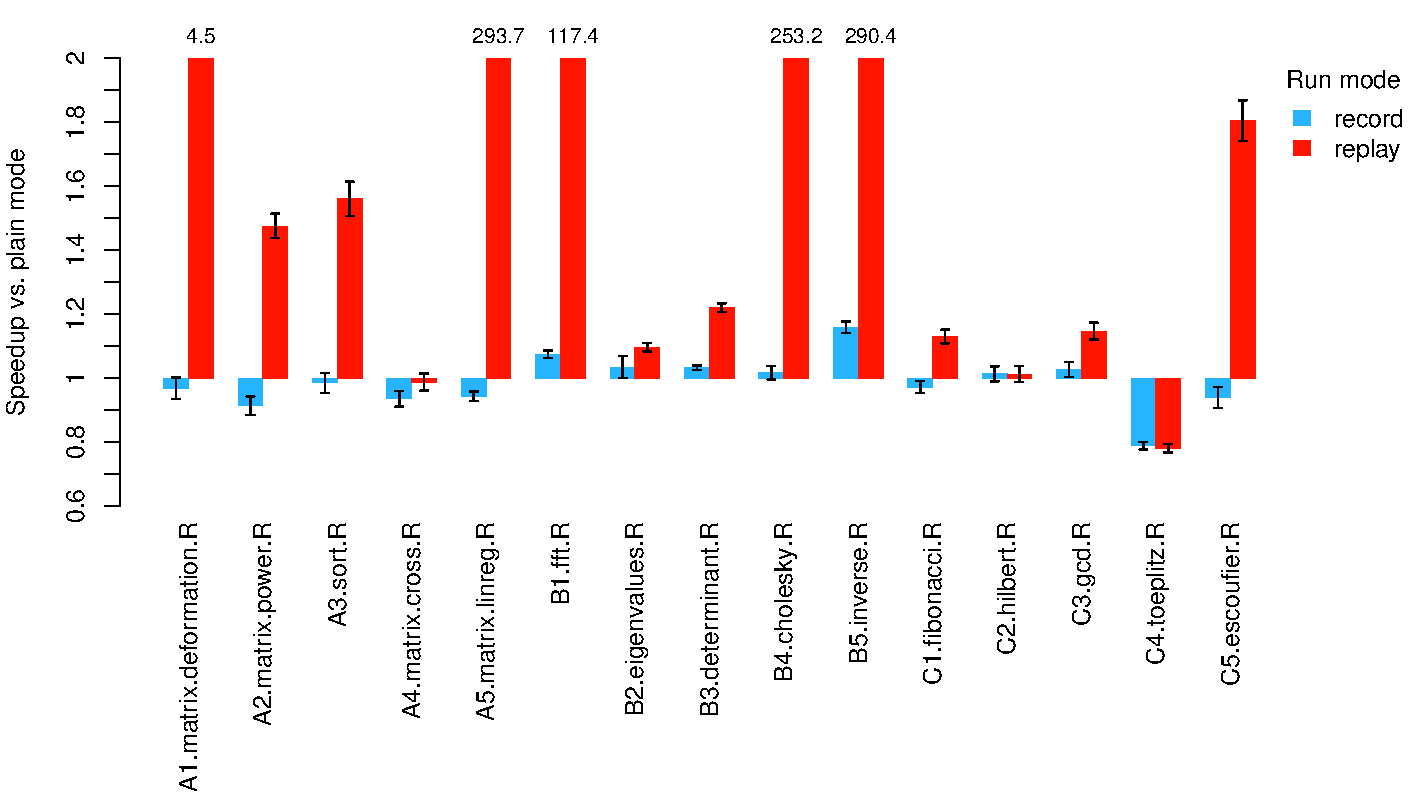
\includegraphics[width=1.0\textwidth]{benchmarks/R-benchmark/plot_difference}
			\caption{Speedup vs. \emph{plain} mode in the R benchmark}\label{fig:rbench_difference}
		\end{figure}
		
		This behaviour is, however, not common to all the tests in the benchmark suite. Some algorithms are implemented directly in R's C code and can be used by calling an internal function. As these algorithms are not non-deterministic the corresponding internal functions are not recorded and therefore the performance benefit is not there. This is for example the case in the test \emph{B2} (using a \lstinline|eigen()| function) which, as a result, does not show any significant speedup or slowdown.\par
		
		The rest of the tests show speedup between -20\% and 90\% which is within expectations. The \emph{C4} test in the \emph{replay} mode is slower than in the \emph{plain} mode which is also as expected, because the slowdown is influenced by the slowdown in the \emph{record} mode. 
		
		In the \emph{record} mode the results are basically ideal. No significant performance impact of the recording can be seen except for the \emph{C4} test which is approximately 33\% slower ($\frac{1}{0.75}$) than in the \emph{plain} mode. The most likely reason for this test to be slower is the amount of calls that must be processed by RRnR during its execution as shown in the table~\ref{fig:rbench_invokes}.\par
		
		With the amount of over 6 million intercepted calls the overhead of the call processing becomes visible but at the same time the slowdown is not nearly as big as it would have to be in order to make RRnR unusable in this case. The \emph{replay} mode is equally influenced by the call processing and shows basically the same performance.\par
		
		\begin{table}[ht]
			\catcode`\-=12
			\centering
			\setlength\extrarowheight{1mm}
			\renewcommand{\tabcolsep}{3pt}
			\rowcolors{2}{black!00}{black!20}
			\begin{tabularx}{\textwidth}{lRRR}
				\bfseries Test & \bfseries RRnR invokes & \bfseries Internal invokes & \bfseries Trace size\\
				A1 & 31 & 10 & 1\\
				A2 & 27 & 8 & 1\\
				A3 & 30 & 10 & 2\\
				A4 & 32 & 12 & 1\\
				A5 & 493 & 91 & 173\\
				B1 & 5 & 1 & 2\\
				B2 & 62 & 21 & 3\\
				B3 & 17 & 6 & 1\\
				B4 & 553 & 118 & 186\\
				B5 & 481 & 89 & 167\\
				C1 & 16 & 1 & 1\\
				C2 & 31 & 8 & 0\\
				C3 & 102 & 1 & 2\\
				C4 & 6,250,022 & 7 & 0\\
				C5 & 96,996 & 29,281 & 5491\\
			\end{tabularx}
			\caption{Numbers of intercepted and recorded calls by RRnR}\label{fig:rbench_invokes}
		\end{table}
		
		\begin{figure}[ht]\centering
			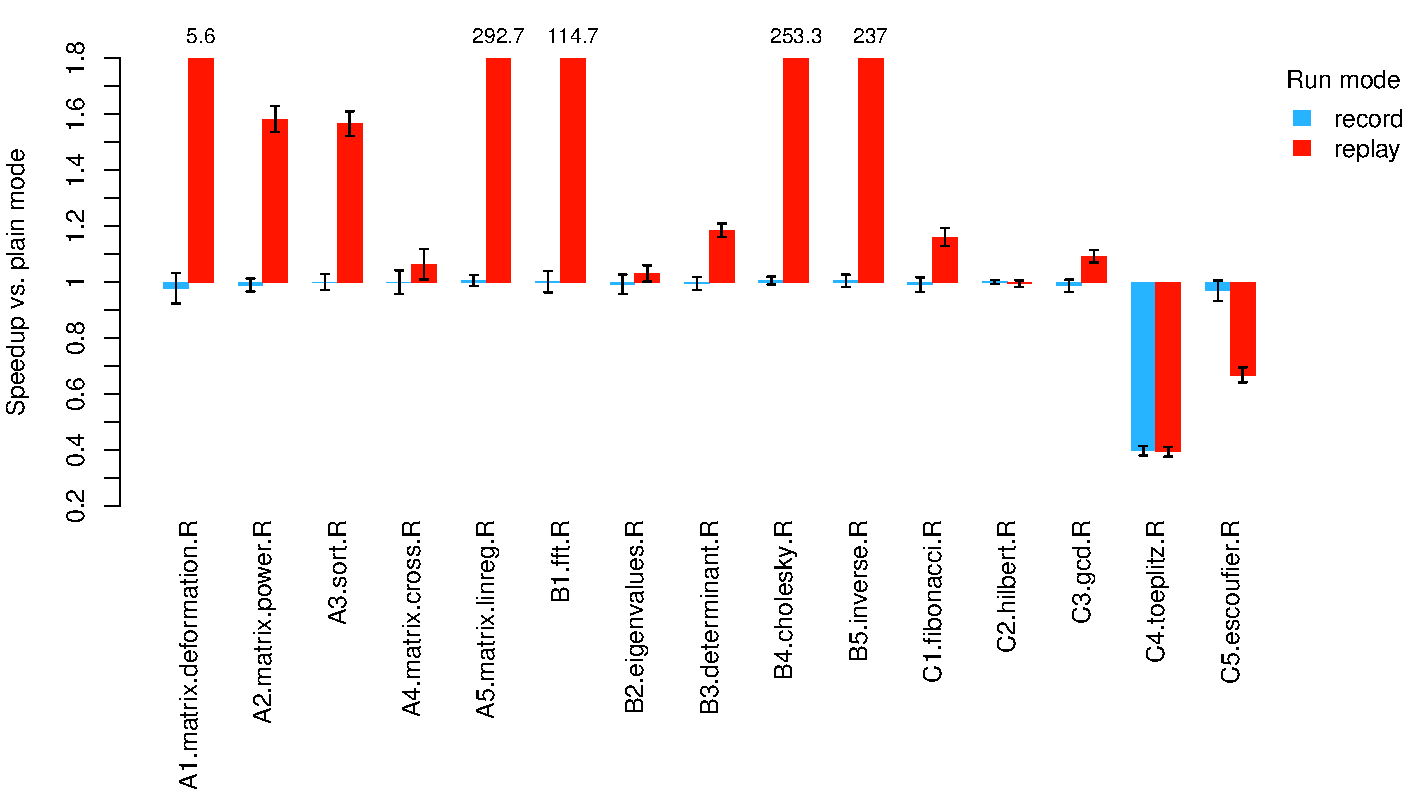
\includegraphics[width=1.0\textwidth]{benchmarks/R-benchmark_orig/plot_difference}
			\caption{Original results without \qt{early-out} for primitives}\label{fig:rbench_orig}
		\end{figure}
		\FloatBarrier
		
		The \emph{RRnR invokes} column in the table shows number of calls processed by RRnR. Every invocation of the \emph{before} handler is counted as one processed call and the handler is invoked whenever there is a call of any builtin or external function.\par
		
		The \emph{Internal invokes} column shows how many of the RRnR invokes are caused by calls of internal functions (the rest is caused by external and primitive function calls). The difference between the first two columns is very important. External calls are all considered non-deterministic and primitive calls are all considered deterministic, therefore they can be processed very quickly. Processing internals, on the other hand, is much slower as their symbols must be compared against the database of non-deterministic internals.\par
		
		The last column shows the final size of the trace which can be also interpreted as an approximate number of the calls which were actually recorded.\par
		
		In the \emph{C4} test out of the 6,250,022 processed calls none is actually recorded. And in the \emph{C5} test, out of the 96,996 processed calls only 5491 are recorded. This may seem very inefficient, however it is important to understand that the only way to detect a non-deterministic call is by processing every single call and make the decision to record it or not based on its properties.\par
		
		During development there was not an \qt{early-out} check for detection of primitives which means that also the symbols of primitive functions were compared against the database. That led to significantly worse performance as shown in the chart~\ref{fig:rbench_orig}. Especially the \emph{C4} test was negatively influenced by the fact that for each of the 6,250,022 calls a search in the database had to be made.\par
		
		By adding the \qt{early-out} for primitives the amount of searches was reduced to just \emph{7} in this case. This optimization was created after evaluating the results of this benchmark by using the table and the chart shown.\par
		
		\subsection{Shootout benchmark}
		The shootout benchmark suite~\cite{shootout} (officially called \emph{The Computer Language Benchmarks Game}) is a set of various computational problems which are used to compare performance of different implementations of the algorithms in different programming languages. The project started in 2002 and was redesigned several times since then. Today it officially supports over 20 languages, however R language is not one of them.\par
		
		The actual implementation of the tests for R was taken from \cite{r_shootout} which is an unofficial port of the shootout benchmark. For each test there are multiple implementations, the ones marked as the fastest were used for this testing.\par
		
		Results of the measurement can be seen in the chart~\ref{fig:shootout_difference}. Generally the shootout benchmark tests showed much larger variation in running time than the R-benchmark tests. This is probably due to the fact that the shootout tests are more complex.\par
		
		\begin{table}[ht]
			\catcode`\-=12
			\centering
			\setlength\extrarowheight{1mm}
			\renewcommand{\tabcolsep}{3pt}
			\rowcolors{2}{black!00}{black!20}
			\begin{tabularx}{\textwidth}{lX}
				\bfseries Test name & \bfseries Description\\
				binary trees & Creation of a perfect binary tree\\
				fannkuch redux & Indexed-access to tiny integer-sequence\\
				fasta native & Generate and write random DNA sequences\\
				fastaredux & Generate and write random DNA sequences\\
				k-nucleotide & Use hash table to count nucleotide sequences\\
				mandelbrot1 & Generate an image of the Mandelbrot set\\
				meteor contest & Find solutions for the Meteor Puzzle\\
				nbody & Double-precision N-body simulation\\
				pidigits & List first N digits of PI\\
				regexdna & Match DNA patterns using regular expressions\\
				revcomp1 & Generate reverse complement of a DNA sequence\\
				spectral-norm-alt & Calculate spectral norm of a matrix\\
			\end{tabularx}
			\caption{Overview of shootout benchmark tests}
		\end{table}
		
		\begin{figure}[ht]\centering
			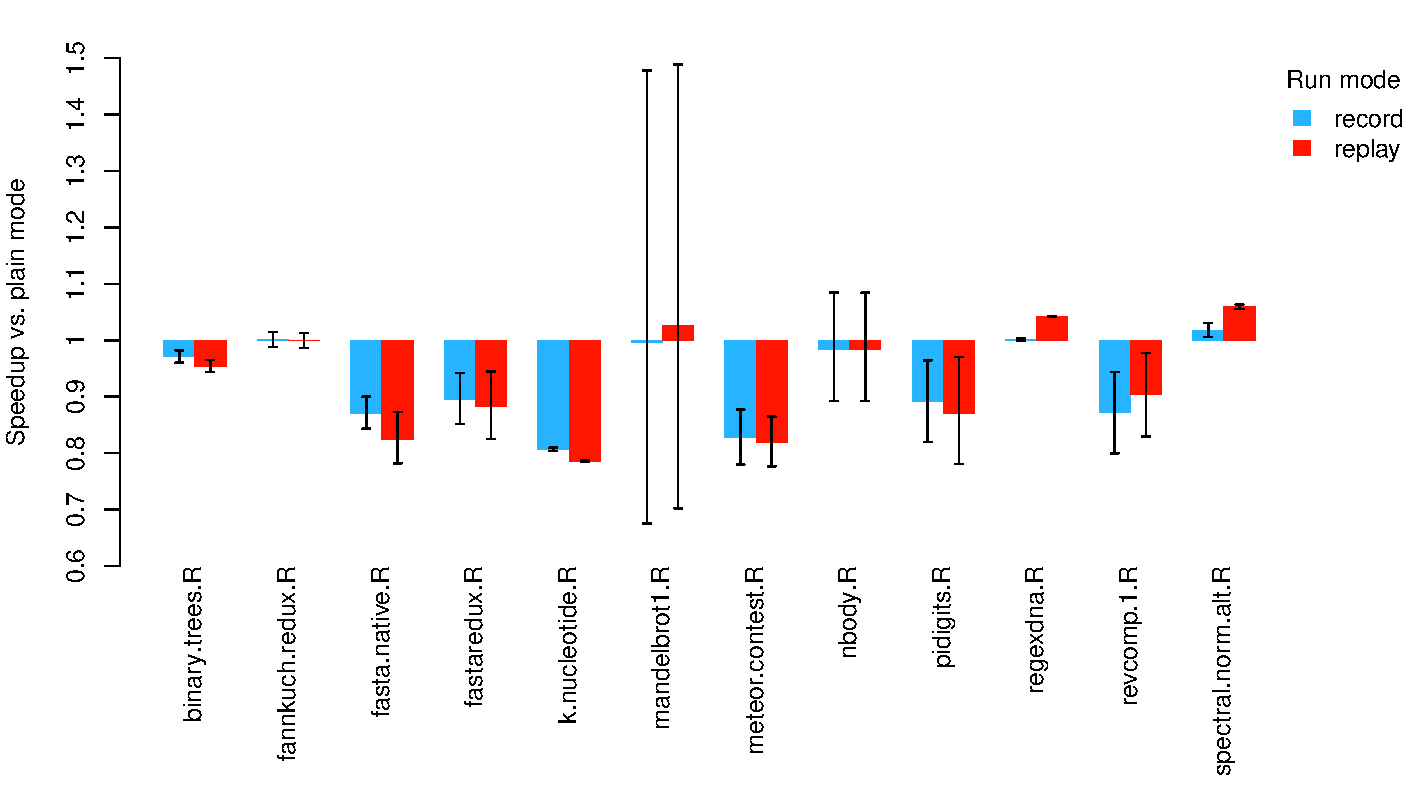
\includegraphics[width=1.0\textwidth]{benchmarks/shootout/plot_difference}
			\caption{Speedup vs. \emph{plain} mode in the shootout benchmark}\label{fig:shootout_difference}
		\end{figure}
		
		The variation in the measured time is so consistent that even at 100 runs per test the results do not converge to a stable value hence the confidence interval spread is quite big, especially in the \emph{mandelbrot} test.\par
		
		The variation is, however, not caused by RRnR as it is also present in the \emph{plain} mode with similar spread.\par
		
		\begin{figure}[ht]\centering
			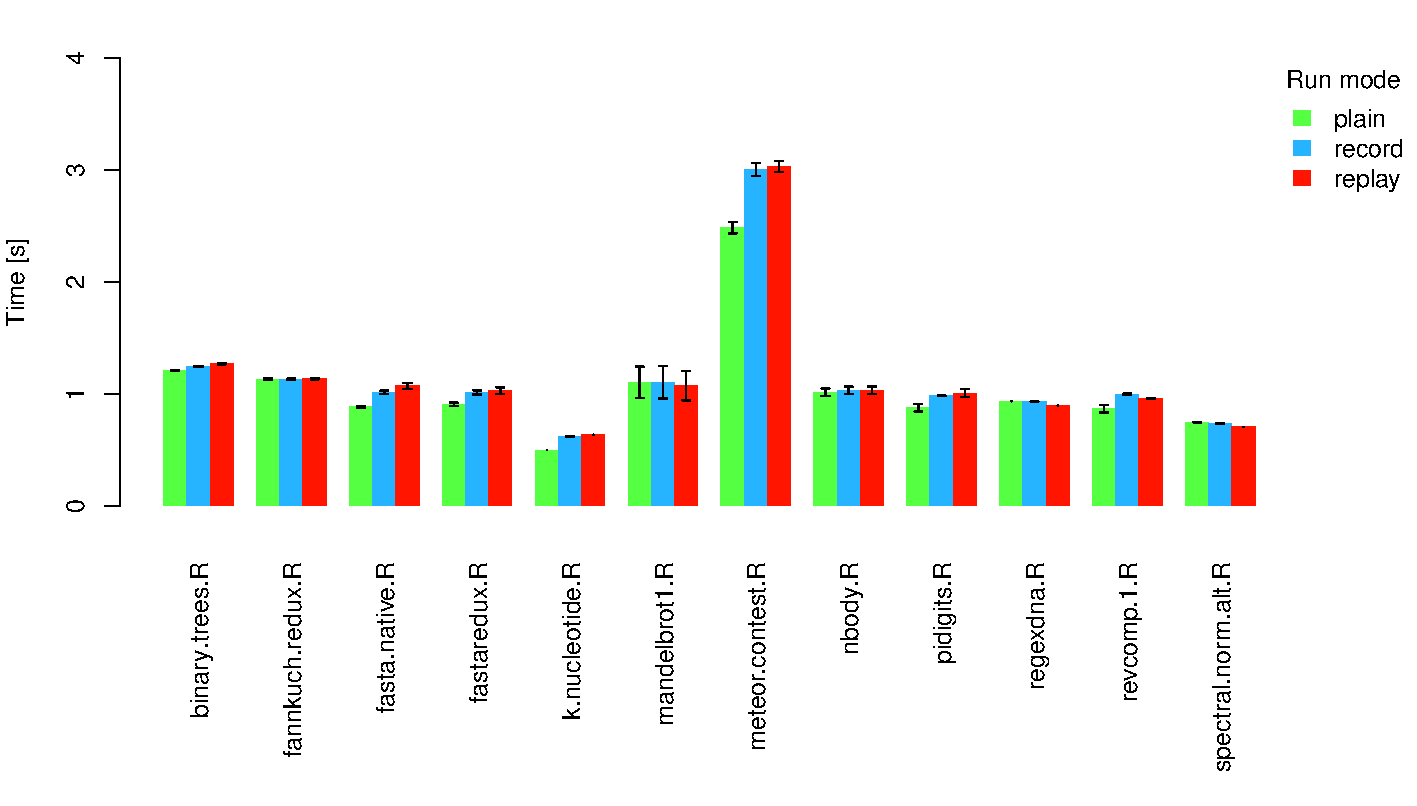
\includegraphics[width=1.0\textwidth]{benchmarks/shootout/plot_running_time}
			\caption{Running time of the tests of the shootout benchmark}\label{fig:shootout_running}
		\end{figure}
		\FloatBarrier
		
		It is also important to note that the confidence intervals in the chart~\ref{fig:shootout_difference} are influenced by the fact that this chart shows ratio of two means where the intervals must be widened in order to keep the 95\% confidence (as described by the Fieller's theorem). The scale of the variations may be better understood when taking into account the actual test running times measured as shown in the chart~\ref{fig:shootout_running}.\par
		
		In most of the tests the \emph{record} mode is on par with the \emph{plain} mode, which is a good result. In some of the tests the \emph{record} mode shows a slowdown within acceptable range, this is the case mainly for the \emph{fasta native}, \emph{k-nucleotide} and \emph{meteor contest} tests. Performance of the \emph{replay} mode is generally the same or slightly faster than the \emph{record} mode.\par
		
		\begin{table}[ht]
			\catcode`\-=12
			\centering
			\setlength\extrarowheight{1mm}
			\renewcommand{\tabcolsep}{3pt}
			\rowcolors{2}{black!00}{black!20}
			\begin{tabularx}{\textwidth}{lRRR}
				\bfseries Test & \bfseries RRnR invokes & \bfseries Internal invokes & \bfseries Trace size\\
				binary trees & 1,324,419 & 14 & 14\\
				fannkuch redux & 2 & 1 & 0\\
				fasta native & 913,386 & 63,350 & 33,342\\
				fastaredux & 1,043,968 & 81,543 & 36,674\\
				k-nucleotide & 562,382 & 281,029 & 377\\
				mandelbrot1 & 43,440 & 15,416 & 2806\\
				meteor contest & 2,493,820 & 1,325,792 & 0\\
				nbody & 480,048 & 5 & 4\\
				pidigits & 3,166,771 & 737 & 108\\
				regexdna & 125 & 53 & 23\\
				revcomp1 & 375,046 & 208,360 & 125,016\\
				spect-norm-alt & 85 & 8 & 2\\
			\end{tabularx}
			\caption{Numbers of intercepted and recorded calls by RRnR}\label{fig:rbench_invokes}
		\end{table}
		
		Unlike the R-benchmark suite the tests of the shootout benchmark are mainly implemented in R code, therefore there is also more calls to be processed (which can be seen in the table~\ref{fig:rbench_invokes}).\par
		
		The difference between the total number of processed calls (RRnR invokes) and the number of internal calls processed (Internal invokes) can be very well demonstrated on the shootout benchmark.\par
		
		The highest number of RRnR invokes is measured in the \emph{pidigits} test, however there are other tests which showed bigger slowdown. That is caused by the fact that these tests (\emph{meteor contest}, \emph{k-nucleotide}) have much higher number of Internal invokes while the \emph{pidigits} test has almost none.\par
		
		\FloatBarrier
		\subsection{Custom micro benchmarks}
		This benchmark suite is designed with the purpose to demonstrate the potential speed benefits of RRnR. It consists of several typical cases where a very slow code can be run very fast during debugging. In a real world scenario the user might benefit from these cases as it would allow him to repeatedly debug the program without the need to wait for the exact same results to be calculated in each run.\par
		
		The first test called \emph{T1-C-sleep} demonstrates a code which runs a slow external C function. Because C functions are never called during replaying the whole C function (sleep in this case) is skipped and its return value is loaded from the trace immediately.\par
		
		The \emph{T2-system-sleep} test is a variation of the first one. This time the external slow code is invoked by a system call \lstinline|system("sleep 1")|. As expected the system call is skipped during replaying.\par
		
		The \emph{T3-download} test downloads a webpage. Because network communication is also a non-deterministic behaviour, it is skipped as well.\par
		
		Finally there is the \emph{T4-big-file} test which is a bit more realistic. It reads a 3 MB file and counts all characters in it. During replaying the filesystem access is completely omitted and the contents of the file are loaded from the trace, which is already in memory, instead. The replaying is \qt{only} two times faster, however with bigger files the speedup would be higher.\par
		
		Although it is worth mentioning that with a really big file, which would not fit in the memory, it would be necessary to enable the \emph{allow\_connections} option which allows direct access to the filesystem even when replaying.\par
		
		\begin{figure}[ht]\centering
			\setlength{\abovecaptionskip}{-5pt}
			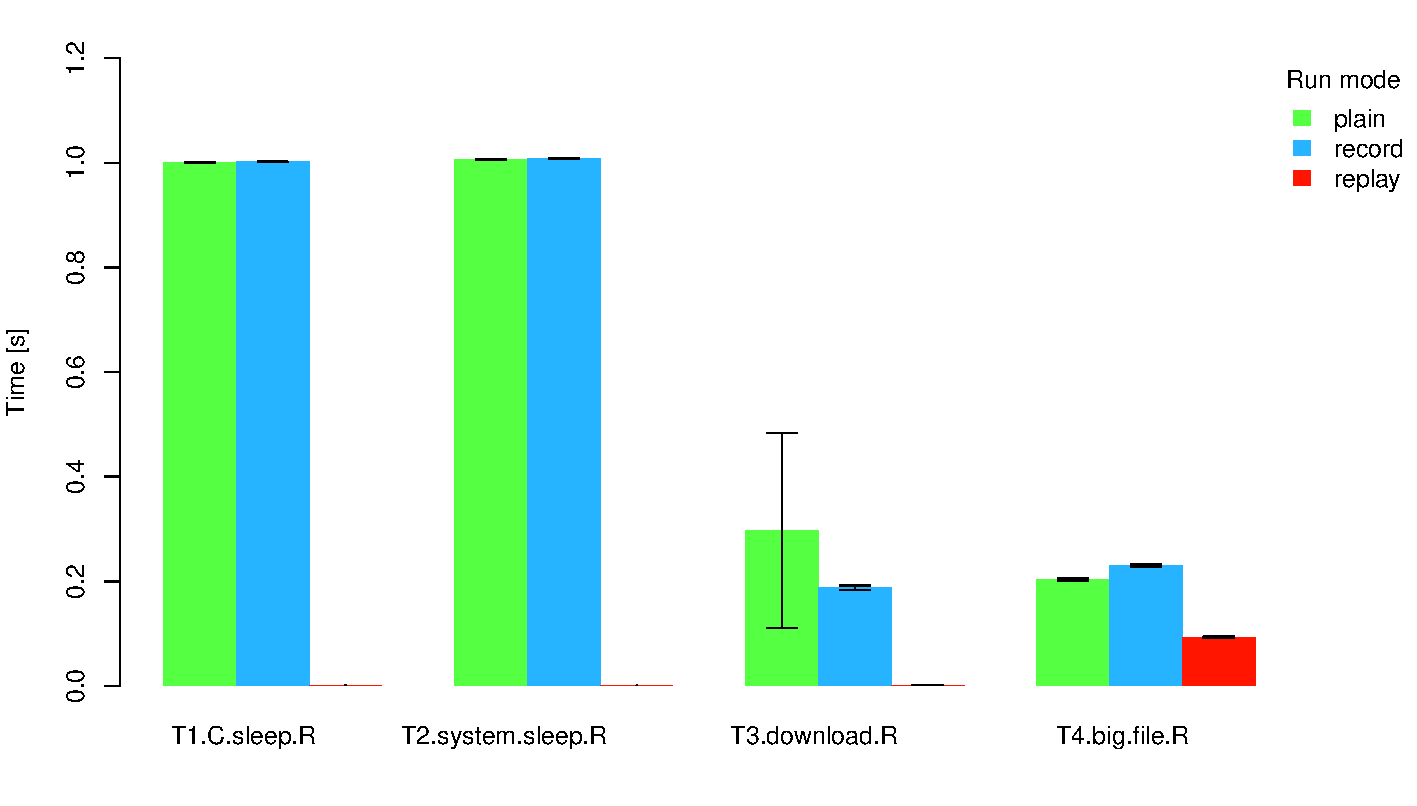
\includegraphics[width=1.0\textwidth]{benchmarks/custom/plot_running_time}
			\caption{Running time of the tests of the custom micro benchmarks suite}
		\end{figure}
	
	\section{Vignette testing}
	A package in R may contain a set of vignettes. Vignettes are a form of documentation that combines interleaved code and text describing the code. The code is runnable and can be extracted. There are thousands of packages available and many of them have vignettes, therefore using them to test RRnR should provide a big picture of what percentage of use cases does RRnR cover.\par
	
	864 vignettes from 456 packages were used in the following scenario -- run the vignette in the \emph{plain} mode three times (to ensure that all caches are filled), then record it once and replay it. Output of the three modes was saved to a file and then compared based on its md5 sum. The \emph{record} mode was considered successful if it produced no error and its output was the same as in the \emph{plain} mode. The \emph{replay} mode was considered successful if it produced no error and its output was the same as in the \emph{record} mode.\par
	
	288 vignettes ended with an error in the \emph{plain} mode so they were excluded from the rest of the testing and also from the results. 9 other vignettes were skipped because they took too much time to compute and two more vignettes (\emph{dlnmTS} and \emph{dlnmExtended}) were skipped because they caused segmentation faults in the \emph{replay} mode. The crash always happened during garbage collection so it is a possible memory protection bug but it has not yet been identified. However, thanks to the vignette testing another bug was discovered and fixed which caused crashes of 10 other vignettes.\par
	
	\begin{figure}[ht]\centering
		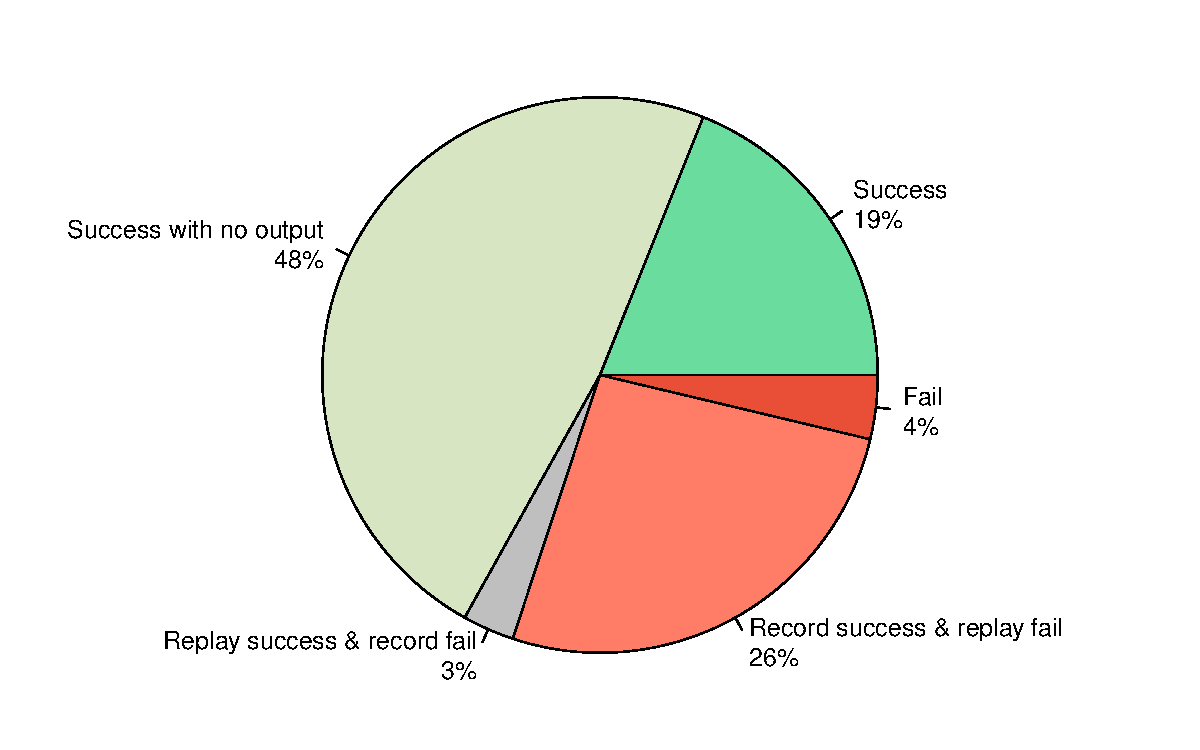
\includegraphics[width=1.0\textwidth]{vignettes/results}
		\caption{Final results of vignette testing}
	\end{figure}
	
	\begin{table}[ht]
		\catcode`\-=12
		\centering
		\setlength\extrarowheight{1mm}
		\renewcommand{\tabcolsep}{3pt}
		\rowcolors{2}{black!00}{black!20}
		\begin{tabularx}{\textwidth}{lRRR}
			Total vignettes used & 864 &\\
			Vignettes skipped & 11 / 864 & 1.3\% \\
			Failed in plain mode & 288 / 864 & 33.3\% \\
			Vignettes tested & 565 / 864 & 65.4\% \\
			Record success & 527 / 565 & 93.3\% \\
			Replay success & 395 / 565 & 69.9\% \\
			Record fail, Replay fail & 21 / 565 & 3.7\% \\
			Record success, Replay fail & 149 / 565 & 26.4\% \\
			Record fail, Replay success & 17 / 565 & 3.0\% \\
			Success & 378 / 565 & 66.9\% \\
			Success with output & 107 / 378 & 28.3\% \\
			Success with trace & 378 / 378 & 100.0\% \\
			Success with output and trace & 107 / 378 & 28.3\% \\
		\end{tabularx}
		\caption{Detailed results of vignette testing}
	\end{table}
	\FloatBarrier
	\pagebreak
	
	Testing of the remaining 565 vignettes had the following outcomes:
	\begin{itemize}
		\item \emph{Success} -- these vignettes succeeded in both the \emph{record} and the \emph{replay} modes and had some output. This means that the success of the tests is backed by a strong evidence that the output of the \emph{replay} mode was the same as the output of the \emph{plain} mode.
		
		\item \emph{Success with no output} -- these vignettes also succeeded in both modes but they had no output, therefore their success is \qt{only} backed by the fact that there was no wrong additional output while replaying. However, all of the successful tests generated a non-empty trace which means that RRnR features were used during all these tests, even during those with no output.
		
		\item \emph{Replay success \& record fail} -- the output of the \emph{record} mode was different than the output of the \emph{plain} mode but the output of the \emph{record} mode was successfully replayed in the \emph{replay} mode. The failure in the \emph{record} mode can be caused by either an error in RRnR, error in the vignette or by random output of the vignette. After investigation it turned out that all of the vignettes in this category have random output (which causes the output comparison to fail) except for one case. And since the replaying worked without a problem these tests can be considered mostly successful.
		
		\item \emph{Record success \& replay fail} -- these vignettes were successfully recorded (no errors, same output as the \emph{plain} mode) but the replay had different output. These failures were probably caused by unhandled corner cases and therefore could be fixed during future development.
		
		\item \emph{Fail} -- these vignettes failed in both the \emph{record} and the \emph{replay} modes. The failures in the \emph{record} mode were in most cases (16 out of 21) caused by a random output of the vignettes. The failures in the \emph{replay} mode were also most likely caused by unhandled corner cases.
	\end{itemize}

	\section{Example usage}
	This section presents the usage of RRnR on an example program shown in the Introduction (\hyperref[example_program]{Listing 1}) which computes average tangent of a given series of angles in degrees. The program works as expected but under some rare conditions it has an unexpected output \lstinline|Inf|.\par
	
	First it is necessary to record the program while the bug is visible. Because the bug has a low probability of appearance, it takes a lot of runs to experience it. Therefore the best approach is to keep recording the program in a loop until the bug is discovered.\par
	
	RRnR provides a function \lstinline|recordFindBug()| which does exactly that. In order to use it the user must provide a function which can detect the bug based on the program's output. In this case, fortunately, the bug can be detected by a short function and the whole recording process looks like this:\par
	
\begin{lstlisting}[style=filestyle, caption={Recording the bug in the example program}]
program <- # definition of the example program

detect <- function(res) is.infinite(res)
rec <- recordFindBug(program(), detect, options=list(max_time=20))
\end{lstlisting}

	If the bug has been successfully recorded, the \lstinline|rec| contains a valid replay structure. Otherwise it contains \lstinline|NULL|. It may happen that the bug is extremely rare and it would take a long time to capture. In that case it might be necessary to manually set the timeout (as shown in the example), 20 seconds is the default value.\par
	
	After successfully recording the bug the user may start with the debugging. Every time the program is replayed by calling \lstinline|replay(rec)| the bug is there so it can be debugged like a normal deterministic bug. In this case it might be a good idea to insert conditional breakpoint inside the program's loop where the tangent is being calculated. By setting the breakpoint to be triggered only when the tangent is \lstinline|Inf| it should be possible to find out which angle causes the problem.\par
	
\begin{lstlisting}[style=filestyle, caption={The part of interest in the example program}]
for(i in 1:length(angles)) {
  adj <- adjacent(angles[i], 1)
  opp <- opposite(angles[i], 1)
  tan <- tangent(opp, adj)
# Let's insert the breakpoint here!
  tangents[i] <- tan
}
\end{lstlisting}
	
	Breakpoints can be inserted by using RRnR's \lstinline|recordTrace()| function which is an RRnR version of the R's \lstinline|trace()| function. The first argument is the replay structure, the second argument is the name of the function where the breakpoint should be inserted, \lstinline|tracer| contains the code of the breakpoint, \lstinline|at| specifies the position in the function and \lstinline|print=FALSE| removes unnecessary output.\par
	
	After starting the replaying the browser opens once the specified condition \lstinline|is.infinite(tan)| is met. Then by browsing the active variables it turns out that the value of the tangent is indeed infinite, because the 5th angle in the input array has value of 90 degrees, therefore the calculated adjacent side of a triangle has 0 length and the fraction of the opposite and adjacent sides is undefined.\par
	
\pagebreak
\begin{lstlisting}[style=filestyle, caption={Example debugging session}]
> recordTrace(rec, "program", tracer=quote(browser(expr=is.infinite(tan))), at=list(c(8,4,5)), print=FALSE)
> replay(rec)
Called from: eval(expr, p)
Browse[1]> tan
[1] Inf
Browse[1]> angles[i]
[1] 90
Browse[1]> i
[1] 5
Browse[1]> adj
[1] 0
Browse[1]> opp
[1] 1
Browse[1]> opp/adj
[1] Inf
Browse[1]> Q
>
\end{lstlisting}

\setsecnumdepth{part}
\chapter{Conclusion}
The goal of this thesis was to create a tool which would help users of R programming language to find non-deterministic bugs in their programs by recording the execution of a program when the bug is visible and then replaying it later multiple times with the bug always present. Also one of the main requirements was the ability to debug from within the R session, ideally by using the standard debugging tools provided by R.\par

First, the existing solutions for Record and Replay debugging were explored. Also the R language was inspected with the focus on the internals of the interpreter in order to choose the best approach for implementation of the solution.\par

Next, a basic solution was implemented by making necessary modifications to the core R and by creating a new base package containing most of the implementation.\par

After that the solution was improved, so that it could be used in more use cases, by dealing with various corner cases like callbacks from C to R, altering environments, printing or triggering errors.\par

Then the solution was evaluated using benchmarks and real world examples. Benchmarks showed that in most cases the solution has small negative impact on performance in recording mode and often has quite big positive impact on performance while replaying. Real world examples showed that even though the solution does not currently support all possible use cases it still can handle a significant percentage of them.\par

It can be clearly stated that the goal of the thesis was met as the implemented tool works in many non-trivial cases. The thesis also proves that the method used is viable and even though the tool does not yet support all possible use cases it can be further improved to support more of them in the future by extending the current solution.\par

	\section{Future work}
	This final section briefly describes functionality that has not yet been implemented and should be considered as possible future improvement of RRnR.\par
	
	One of the first things to do is focusing on the vignette testing results, especially on the reasons of the \emph{replay} mode failures. Most likely these failures were caused by corner cases which has not yet been handled. Therefore the next step is to create a list of the problems and fix them. As of now the following problems are known.\par
	
		\subsection{Recursive environment cloning}
		If an environment contains another environment then only the outer one is cloned right now. Therefore when a change happens between recording and replaying in the inner environment then the change is not reverted and it might influence the replaying.\par
		
		In order to address this issue it would be necessary to do \emph{recursive cloning} which may be very slow, memory demanding and complex as there would also have to be a circular dependency check.\par
		
		\subsection{Support for S4 methods}
		The \emph{methods} package uses class caches, method tables and other structures which cause additional code to be executed along with the program being recorded. It must be ensured that always the same code is executed in recording and replaying runs.\par
		
		\subsection{Recursive in-trace replacement}
		The environment in-trace replacement now works only for environments which are stored \emph{directly} in the trace. But this process should work recursively even for environments which are stored inside a data structure which is stored in the trace.\par
		
		\subsection{Reverse execution}
		Finally there is a feature that might be implemented in order to enhance the RRnR functionality. It is the ability to reverse-execute a program which is a big feature of the Mozilla rr. It means that during debugging it is not only possible to step forward but also to step backward.\par
		
		Such feature can be implemented by creating snapshots of the program's state during its execution, then loading the latest snapshot before the current position and stepping forward until the desired position in code is reached.\par
		
		Usefulness of this function is apparent as it is beneficial to be able to step through the code back and forth as needed in order to discover a bug.\par

\bibliographystyle{iso690}
\bibliography{bibliography}

\setsecnumdepth{all}
\appendix

\chapter{Implementation overview}

\begin{figure}[ht]\centering
	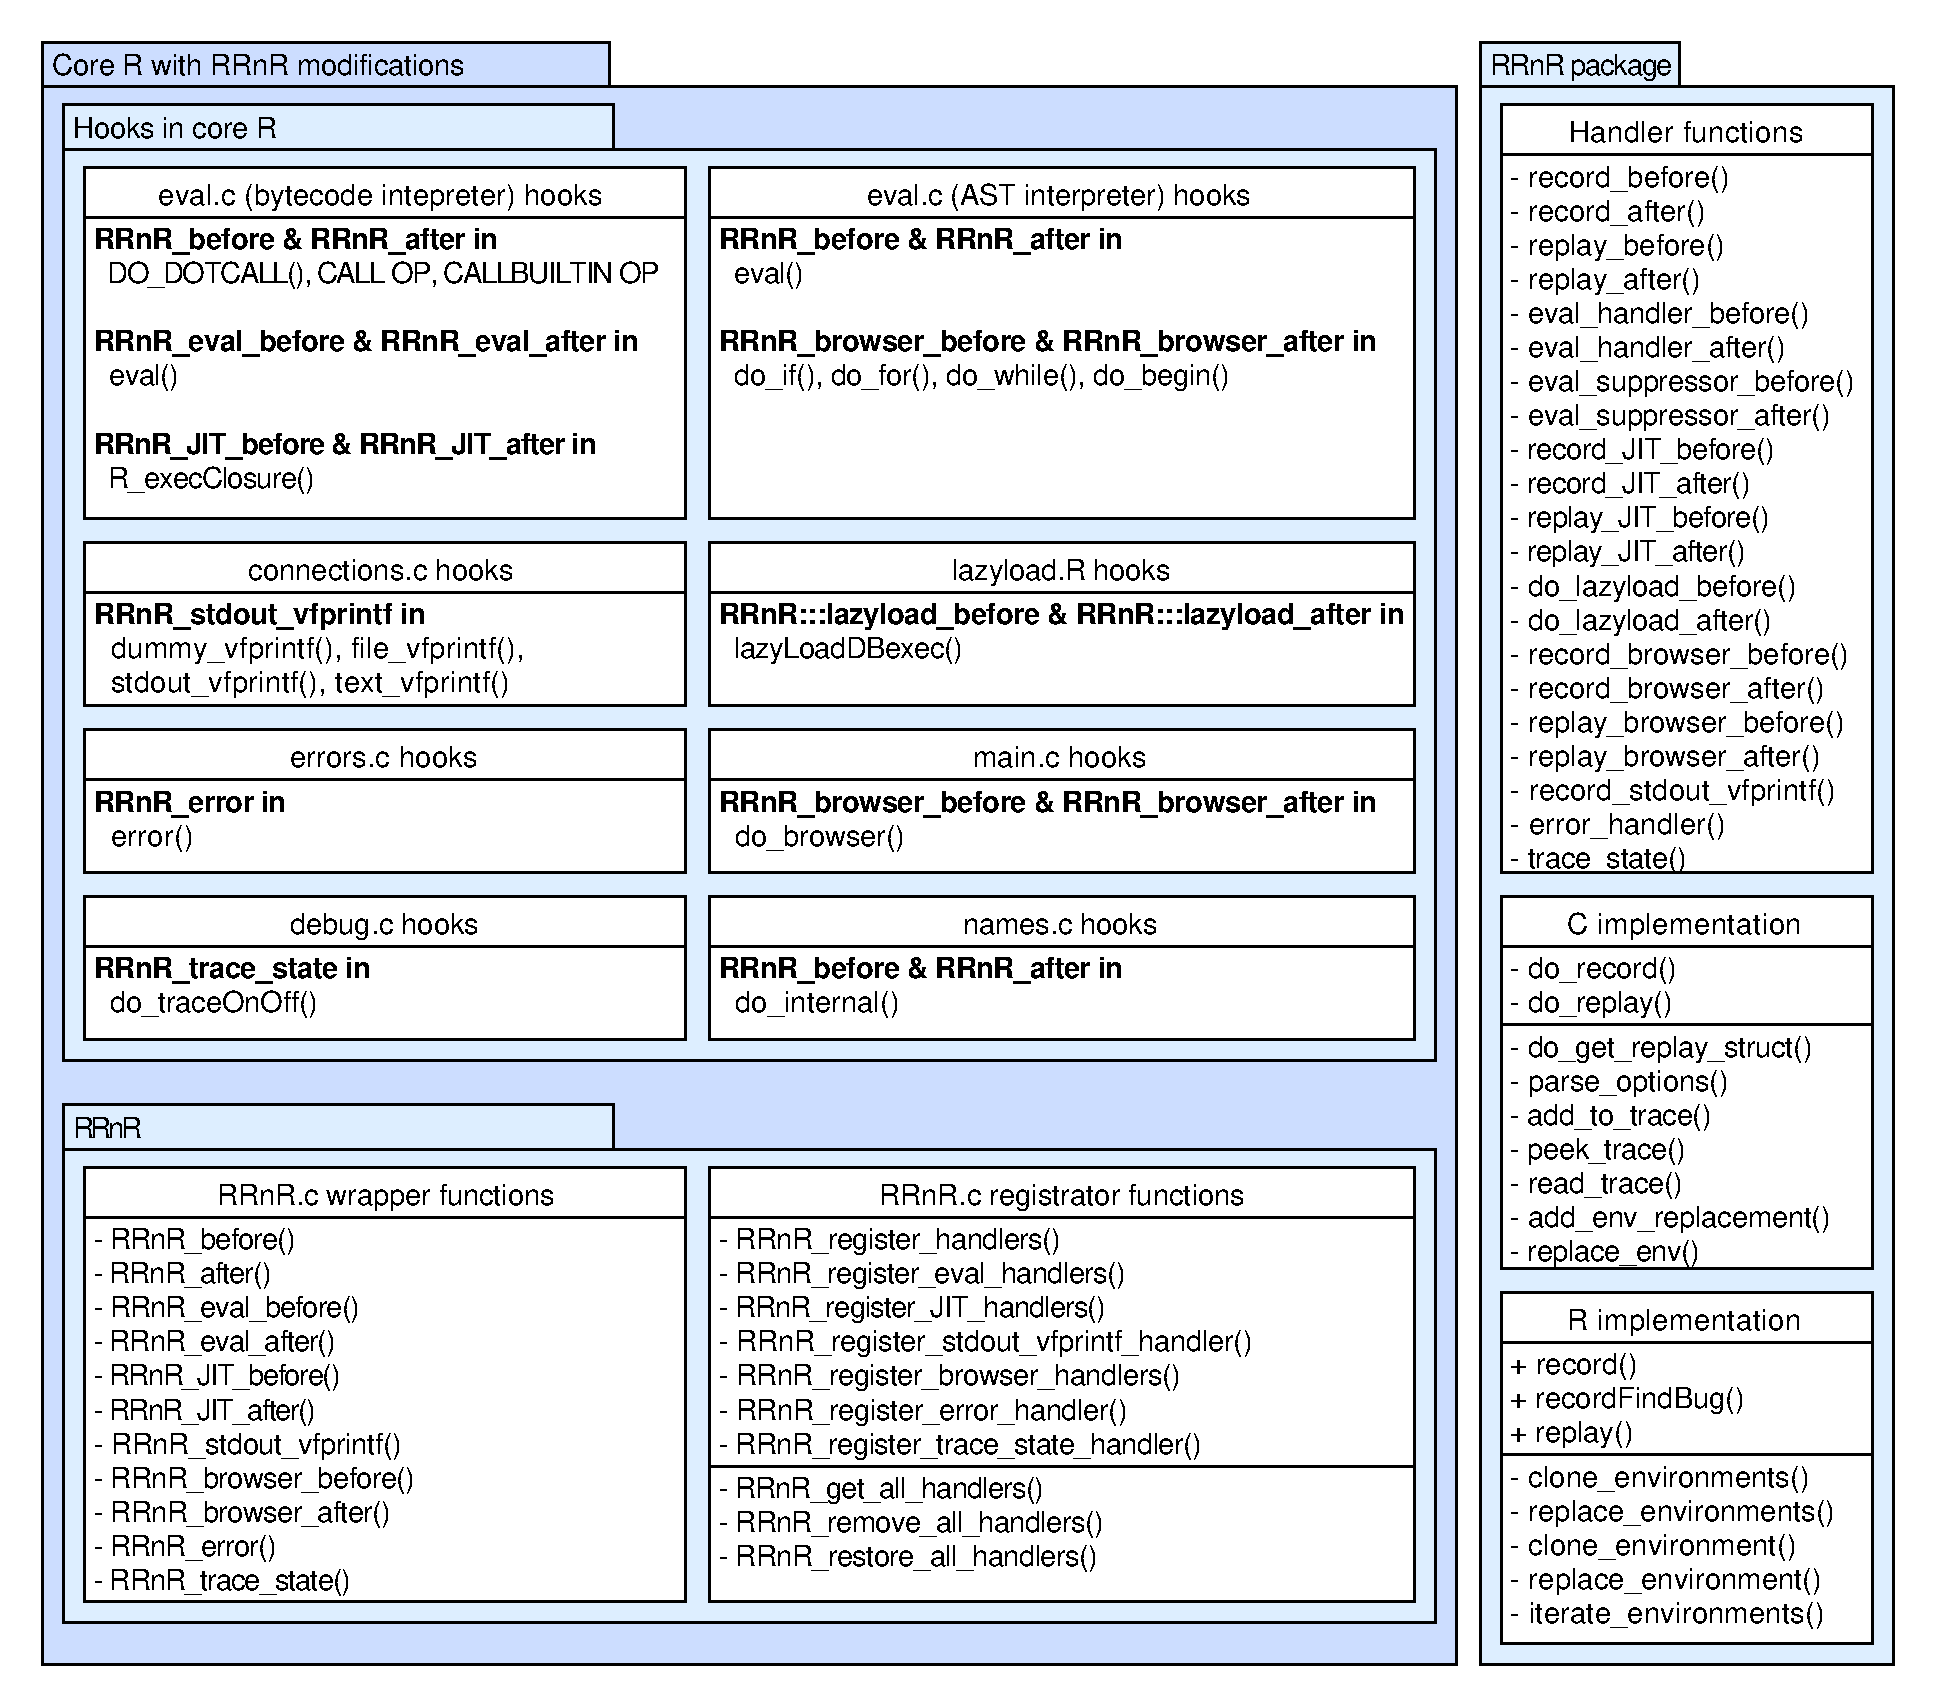
\includegraphics[width=1.0\textwidth]{img/incorporation_into_r}
	\caption{Overview of additions and modifications made during implementation}\label{fig:incorporation_into_r}
\end{figure}

\chapter{Contents of enclosed DVD}

%change appropriately

\begin{figure}
	\dirtree{%
		.1 Thesis.pdf\DTcomment{the text of the thesis}.
		.1 thesis\_src\DTcomment{\LaTeX{} source code of the thesis}.
		.2 Makefile\DTcomment{use \lstinline|make all| to create PDF from the source}.
		.2 latex\_src/benchmarks\DTcomment{benchmark result data}.
		.2 latex\_src/vignettes\DTcomment{vignette testing result data}.
		.1 modified-R\DTcomment{fork of R 3.4.3 with the RRnR implementation}.
		.2 configure\DTcomment{use \lstinline|./configure| to prepare Makefile}.
		.2 Makefile\DTcomment{use \lstinline|make| to compile the modified R}.
		.2 bin/R\DTcomment{the compiled executable}.
		.2 src/library/RRnR\DTcomment{the RRnR package source code}.
		.1 results\DTcomment{raw results of the benchmarks and the vignette testing}.
	}
\end{figure}

\end{document}
